\section{Experimente - Durchführung}\label{hauptabschnitt_5}
\paragraph{Motivation}\label{par_EXP_durch_motiv}

Die in Kapitel \ref{hauptabschnitt_2} erwähnten Experimente der Arbeit \cite{dubey2018investigating} bieten unausgeschöpftes Potential zur Evaluation der Generalisierung eines RL-Agenten. So kann bspw. durch die Maskierung der Information der Orbs getestet werden, wie wichtig diese Information für den erfolgreichen Abschluss eines Levels ist. Darüber hinaus kann man damit ermitteln, ob der Agent etwas über die zugrunde liegende Level-Struktur bzw. den Algorithmus der die Level erstellt, lernt oder das gesamte Konzept des Spiels verstanden hat. Darüberhinaus wird untersucht, ob die Orbs dem Agenten nach einer gewissen Trainings-Dauer keinerlei wichtige Information mehr bieten. 

Viele DRL-Agenten, die im Rahmen von Arcade-Spielen eingesetzt werden, bekommen den Bildschirm-Output des jeweiligen Spiels in Form eines ein- oder zwei-dimensionalen Arrays als Input. Somit ist alles was der Agent bisher an Stimuli erhalten hat lediglich ein Array mit ein oder zwei Dimensionen. Nimmt man nun in einer Evaluation Änderungen am Environment vor, kann das radikale Auswirkungen auf die Performance des Agenten haben. 


\subsection{Zu beantwortende Fragen}\label{subsec_EXP_durch_fragen}
Unter den bisher beschriebenen Umständen wurden für diese Arbeit folgende Sets an Fragen entwickelt, die über den Verlauf der Experimente beantwortet werden. \\
Das erste Set reproduziert die Ergebnisse aus dem Procgen-Paper \cite{cobbe2019procgen} und untersucht die Auswirkung von prozeduraler Level-Erstellung auf die Performance von Agenten. Dieses Set dient hauptsächlich der Bestätigung der Korrektheit der Implementierung.\\
Das zweite Set befasst sich mit visuellen Veränderungen der Farbe der Orbs und des Hintergrundes, aber auch mit Maskierungen gewisser visueller Information. \\
Das dritte Set befasst sich ausschließlich mit semantischen Veränderungen, wie das Tauschen von zwei Sprites.

\paragraph{Set 1 - Reproduktion und Generalisierung}\label{par_EXP_durch_fragen1}
\begin{itemize}
  \item Lassen sich die Ergebnisse aus dem Paper \cite{cobbe2019procgen} mit den eingesetzten Mitteln reproduzieren?
  \item Wie wirkt sich die prozedurale Erstellung und die daraus folgende hohe Diversität der Level auf die Generalisierung und die Sample Efficiency aus?
  \label{lst:itemList_EXP_durch_fragen1}
\end{itemize}
\paragraph{Set 2 - Farbliche Änderung}\label{par_EXP_durch_fragen2}
 \begin{itemize}
  %\item Wie wirkt sich die prozedurale Erstellung und die daraus folgende hohe Diversität der Level auf die Generalisierung und die sample efficiency aus?
  \item Wie wirkt sich das Fehlen visueller Orb-Information auf die Performance aus? 
  \item Wurde das Konzept eines Orbs verstanden? Wirken sich Änderungen der Farbe der Orbs negativ aus? 
  \item Wie viele Level können mit der verwendeten Architektur auswendig gelernt werden? Welche Rolle spielt die visuelle Orb-Information dabei? 
  \label{lst:itemList_EXP_durch_fragen2}
\end{itemize}

\paragraph{Set 3 - Semantische Invertierung}\label{par_EXP_durch_fragen3}
\begin{itemize}
  \item Wie wirkt sich das Tauschen der Sprites von kleinen Orbs und Mauern aus?
  \item Wie wirkt sich das Tauschen der Sprites von großen Orbs und Geistern aus? \\ 
  \label{lst:itemList_EXP_durch_fragen3}
\end{itemize} 

Das genau Setup bezüglich Dauer des Trainings oder Anzahl der trainierten Level etc. ist tabellarisch bei den jeweiligen Experimenten definiert. 
Generell wird die Leistung der Agenten mit einer \dq one-shot\dq -Evaluation bewertet. Das bedeutet, dass die Episode, während der Evaluation eines Levels, keine Zeitbeschränkung hat und kein Level ein zweites Mal dran kommt. Weiter wird standardmäßig auf 50 unbekannten Leveln trainiert. Änderungen an diesem Vorhaben werden in den jeweiligen Experimenten erläutert. Die Abkürzung SW steht folgend für Sliding Window. 

\paragraph{Farbliche Distanz}\label{farblicheDistanz}
Fortan definiert der Begriff der \emph{farblichen Distanz} die Entfernung zweier Farben zueinander, in einem dreidimensionalen Farbraum. Diese Distanz misst also die absolute Differenz der jeweiligen RGB-Farben. So haben die Farben Rot (r:255, g0:, b:0) und die Farbe Blau (r:0, g0:, b:255) eine farbliche Distanz von $510$. Von rot zu blau muss der Rot-Wert der Farbe auf $0$ und der Blau-Wert auf $255$ gesetzt werden ($|-255| + |255| = 510$). So ergibt sich für die Farben Schwarz und Weiß eine farbliche Distanz von $765$.

\subsection{Reproduktion der Ergebnisse von Procgen}\label{sec:absch_EXP_durch_reproduktion}
Bevor die Experimente der jeweiligen Sets evaluiert werden können, muss die Frage beantwortet sein, ob die verwendeten Implementierungen in der Lage sind, die Ergebnisse aus dem Paper zu reproduzieren, welches dem Environment zugrunde liegt. Im Paper \cite{cobbe2019procgen}~[S.7-8] wird unter dem Punkt 3.3 eine Untersuchung vorgestellt, deren RL-Agent für eine Dauer von 200 Mio. Zeitschritten in 500 Leveln trainiert wird. Dieser Agent wurde ebenfalls mit der in dieser Arbeit verwendeten IMPALA-Architektur \cite{espeholt2018impala} trainiert. 

Das beschriebene Experiment wird in einem kleineren Rahmen, unter denselben Bedingungen durchgeführt. Genauer wird ein Agent für 80 Mio. Zeitschritte in 200 Leveln trainiert. Dies entspricht einer Skalierung der ursprünglichen Dauer und Größe des Experiments von $\frac{2}{5}$. Einen Blick auf den Input des Agenten dieses Experiments liefert Abbildung \ref{fig:pic_chaserKlein}.

\begin{figure}[htp!]
   \centering
   \captionsetup{width=0.48\linewidth} 
    \begin{minipage}{0.48\linewidth}
        %\centering
        \textbf{Training}\par\medskip
        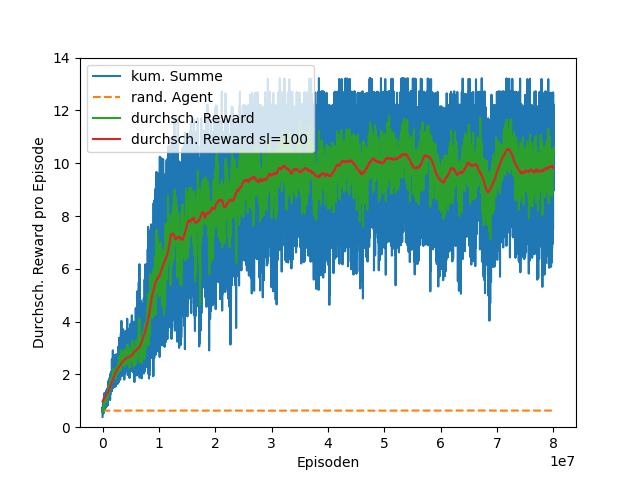
\includegraphics[scale=0.49]{abb/_graphen/floor_80Mio_200lvl_15act_Training}
        \caption{Blau: kumulierter Reward; Grün: durchschnittlicher kumulierter Reward; Rot: Grün mit SW 100; Orange: rand. Agent.}
        \label{fig:grph_floor_80Mio_200lvl_15act_Training}
    \end{minipage}
    \centering
    \begin{minipage}{0.48\linewidth}
        %\centering
        \textbf{Evaluation}\par\medskip
        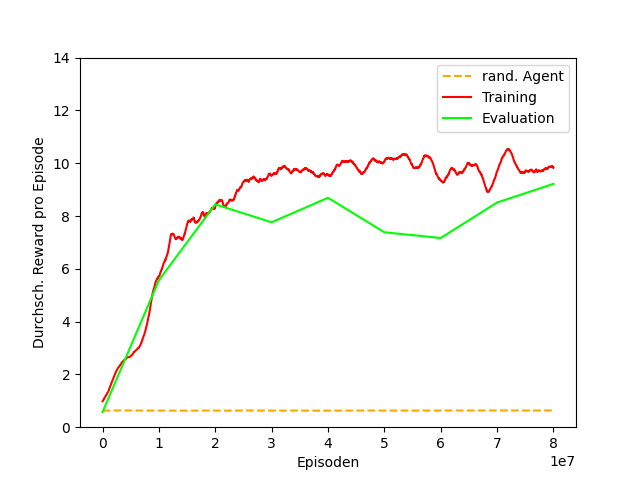
\includegraphics[scale=0.5]{abb/_graphen/floor_80Mio_200lvl_15act_Training_evalAsTraining}
        \caption{Evaluation: one-shot, 50 Level, 8 Checkpoints des Trainings.}
        \label{fig:grph_floor_80Mio_200lvl_15act_evalAsTraining}
        \hfil
    \end{minipage}
\end{figure}

\begin{center}
 \begin{table}[htb!]
 \begin{center}
  \begin{tabular}{ l c c c c }
    \hline
		      & Zeitschritte & Anzahl Level & Hintergrund & Farbe Orb \\ \hline \hline
     Training     & 80 Mio       & 200		 & 	    normal & r:0, g:255, b:0 \\ \hline
     Evaluation & - 	           & 50		 & 	    normal & r:0, g:255, b:0 \\ \hline
    \hline
  \end{tabular}
  \caption{Übersicht über geltende Rahmenbedingungen in Training und Evaluation - 1.}
  \label{tab:tab_durch_EXP_trainSetting1}
  \end{center}
 \end{table}
\end{center} 

Tabelle \ref{tab:tab_durch_EXP_trainSetting1} zeigt die geltenden Rahmenbedingungen während des Trainings. Die linke Abbildung (\ref{fig:grph_floor_80Mio_200lvl_15act_Training}) zeigt eine detaillierte Übersicht über das Training des Agenten. In blau wird der kumulierte Reward angegeben. Der grüne Graph gibt den durchschnittlichen kumulierten Reward an und der rote Graph zeigt den durchschnittlichen kumulierten Reward mit einem SW von 100. Die rechte Abbildung (\ref{fig:grph_floor_80Mio_200lvl_15act_evalAsTraining}) zeigt eine Evaluation von acht Checkpoints über den Verlauf des Trainings. Gemessen wird die one-shot Performance des Agenten in 50 ungesehenen Leveln pro Checkpoint. Jeder Checkpoint wird in denselben 50 Leveln evaluiert. Die Evaluation findet, abgesehen von den ungesehenen Leveln, unter Trainingsbedingungen statt. 

\begin{figure}[htb!]
    \begin{minipage}{\linewidth}
        \centering
        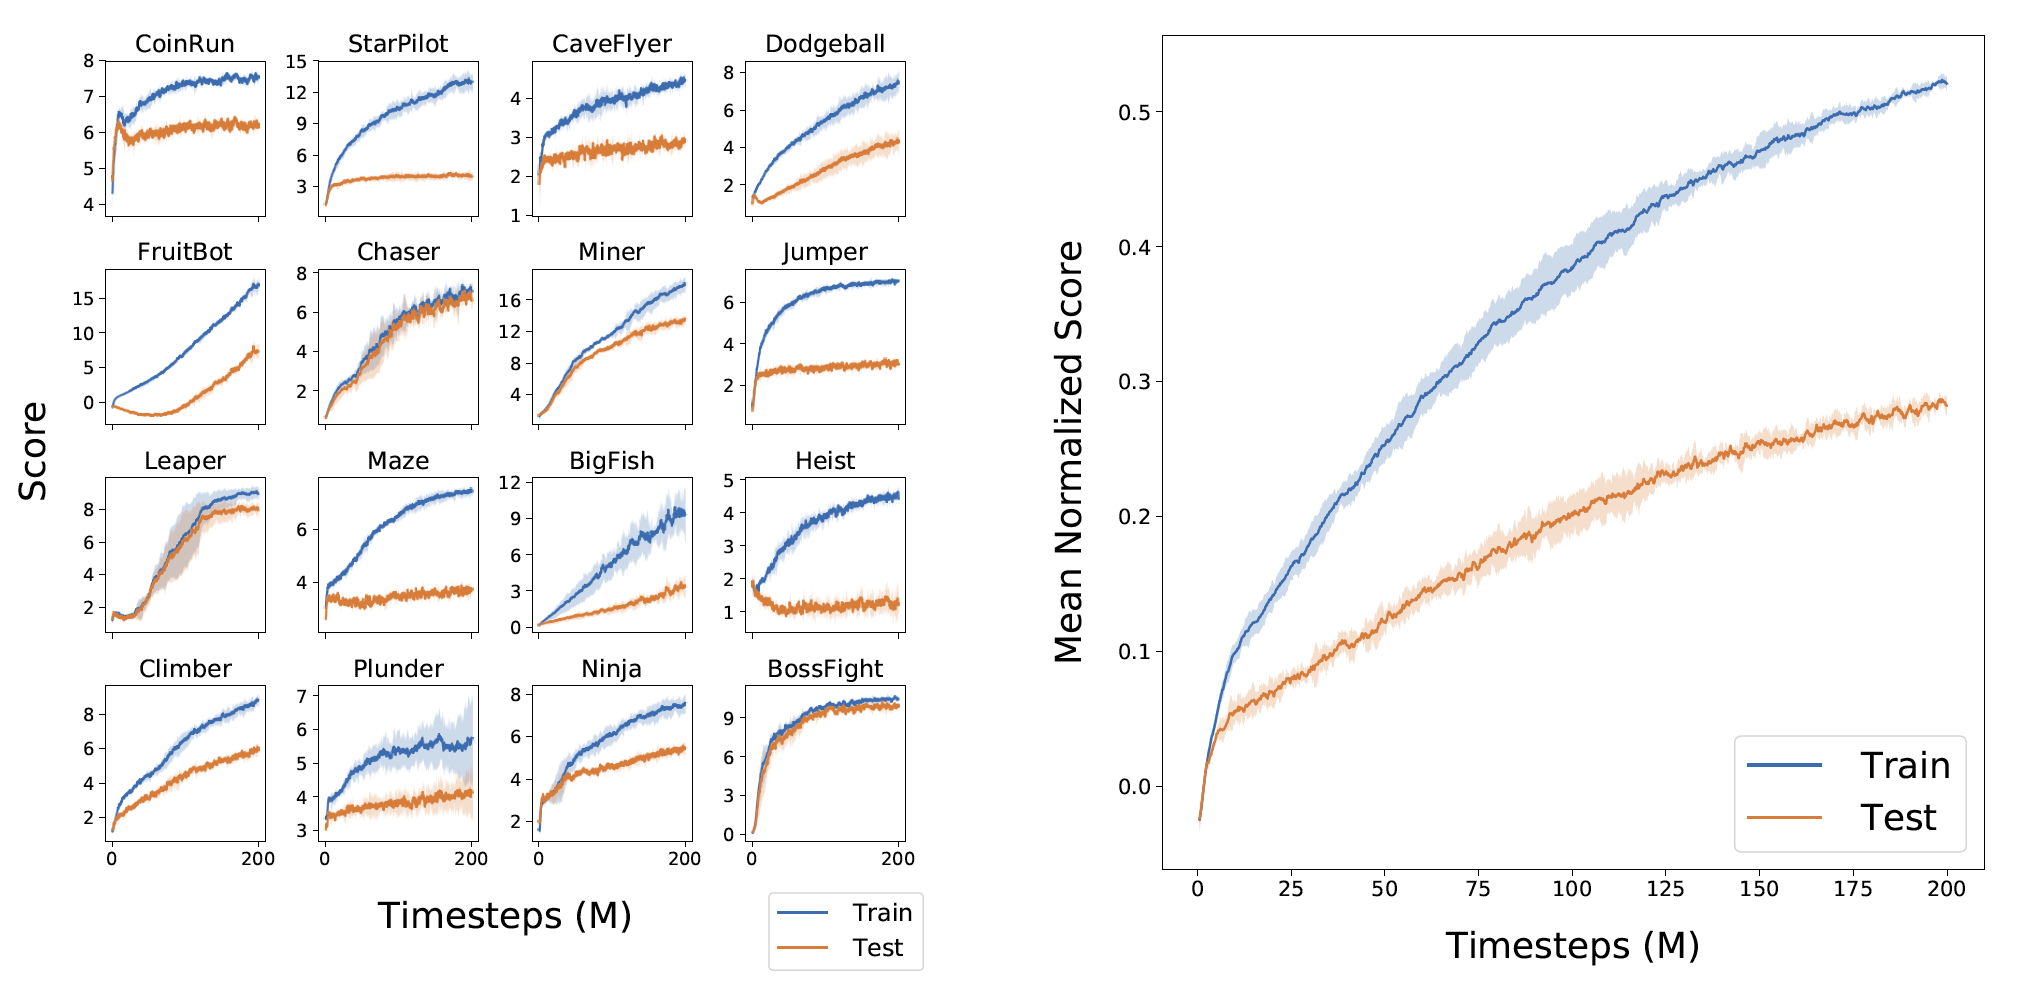
\includegraphics[scale=0.4]{abb/_graphen/procgen_fig4}
        \caption{Experiment zur Generalisierung des Procgen-Papers für 200 Mio. Zeitschritte, in 500 Leveln \cite{cobbe2019procgen}.}
        \label{generalization_500lvl_procgen}
    \end{minipage}
\end{figure}



\textbf{Diskussion:} Ein Vergleich zwischen der Abbildung \ref{fig:grph_floor_80Mio_200lvl_15act_evalAsTraining} und der Abbildung \ref{generalization_500lvl_procgen} zeigt, dass die Ergebnisse nicht nur reproduzierbar sind, sondern mit den eingesetzten Mitteln sogar übertroffen werden können. Im Paper von Procgen endet der Trainingsgraph von Chaser nach 500 Leveln, bei 200 Mio. Zeitschritten, bei einem Reward von etwa $7,2$ (vgl. \ref{generalization_500lvl_procgen}). Beim Reproduktions-Experiment wird nach 200 Leveln bei 80 Mio. Zeitschritten, ein Reward von etwa $9,8$ erreicht. Eine mögliche Erklärung für diese Diskrepanz ist die fehlende Angabe zum eingesetzten Skalierungsfaktor der IMPALA-Architektur für dieses Experiment. Der Vergleich der Ergebnisse in Abbildung \ref{fig:grph_floor_80Mio_200lvl_15act_evalAsTraining} mit der Abbildung \ref{generalization_500lvl_procgen} suggeriert jedoch, dass die Autoren an dieser Stelle eventuell einen kleineren Skalierungsfaktor, bspw. 2 statt 4, für die Architektur verwenden. Eine weitere mögliche Erklärung für die niedrigere Performance im Procgen-Paper könnte sein, dass über mehrere Seeds hinweg evaluiert wird und dass die Seeds der Autoren schwieriger sind, als der Seed, welcher in dieser Arbeit verwendet wird. Hierzu bietet die Arbeit \cite{cobbe2019procgen} jedoch ebenso keinen Hinweis. Die Abbildung Chaser im Procgen-Paper (\ref{generalization_500lvl_procgen}) zeigt auf, dass nahezu keine Generalisierungslücke zwischen Training und Evaluation besteht. Das bedeutet, dass der Agent über den Verlauf dieses Trainings generalisieren kann. Dieser Fakt kann ebenfalls reproduziert werden. Abbildung \ref{fig:grph_floor_80Mio_200lvl_15act_evalAsTraining} zeigt, dass wie im Paper fast keine Generalisierungslücke besteht. Der Leistungseinbruch bei den Checkpoints 50 Mio. und 60 Mio. ist im Rahmen der erwarteten Varianz von DRL. 

\paragraph{Antwort: Set 1, Punkt 1}
Somit kann in $\frac{2}{5}$ der Zeit und Level-Anzahl eine zufriedenstellende Reproduktion realisiert werden. Die erste Frage aus Set 1, kann also mit \dq Ja\dq{} beantwortet werden. Dadurch ist die Grundlage geschaffen, um weitere Experimente mit den eingesetzten Implementierungen durchzuführen. 


\subsubsection{Untersuchung zum Beitrag von prozeduraler Generierung bei DRL}\label{subsec:absch_EXP_durch_reproduktion_generalisierung}
\paragraph{Vergleich Level-Anzahl: 200, 1}\label{par:durch_EXP_vgl_200_1}
Der folgende Paragraph vergleicht zwei Agenten, welche sich einzig in der Anzahl der im Training verwendeten Levels unterscheiden.
Abbildung \ref{fig:grph_floor_80Mio_200lvl_15act_evalAsTraining_1} zeigt Training und Evaluation des Agenten, welcher mit einer fixen Anzahl von 200 Leveln trainiert ist. Dies ist derselbe Agent, wie in Abbildung \ref{fig:grph_floor_80Mio_200lvl_15act_Training}. Auf der rechten Seite ist ein weiterer Agent gezeigt. Der neue Agent ist unter denselben Umständen wie der Agent auf der linken Seite trainiert, mit dem Unterschied, dass der rechte Agent auf ein einziges Level im Training beschränkt ist.
\begin{figure}[htp!]
   \centering
   \captionsetup{width=0.45\linewidth} 
    \begin{minipage}{0.48\linewidth}
        \centering\
        \textbf{Level-Anzahl: 200}\par\medskip
        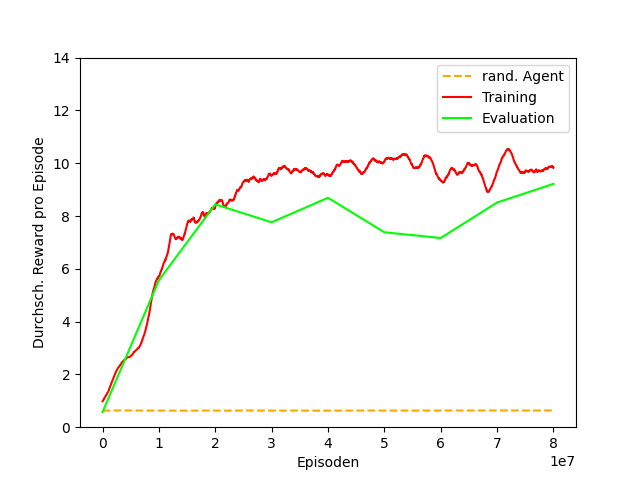
\includegraphics[scale=0.5]{abb/_graphen/floor_80Mio_200lvl_15act_Training_evalAsTraining}
        \caption{Evaluation: one-shot, Training mit fixer Level-Anzahl.}
        \label{fig:grph_floor_80Mio_200lvl_15act_evalAsTraining_1}
    \end{minipage}
    \centering
    \begin{minipage}{0.48\linewidth}
        \centering
        \textbf{Level-Anzahl: 1}\par\medskip
        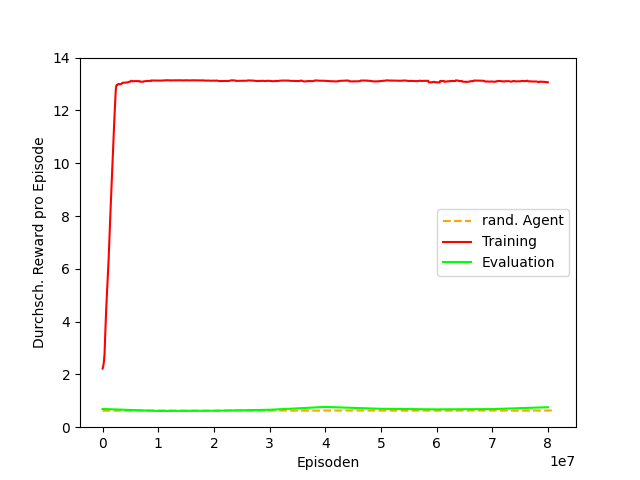
\includegraphics[scale=0.5]{abb/_graphen/floor_80Mio_1lvl_15act_Training_evalAsTraining}
        \caption{Evaluation: one-shot, Training mit unbeschr. Level-Anzahl.}
        \label{fig:grph_floor_80Mio_1lvl_15act_evalAsTraining}
    \end{minipage}
\end{figure}

\begin{center}
 \begin{table}[htb!]
 \begin{center}
  \begin{tabular}{ l c c c c }
    \hline
			       	& Zeitschritte 	& Anzahl Level 	& Hintergrund 	& Farbe Orb \\ \hline \hline
     Level-Anzahl 200 	& 80 Mio       	& 200		& 	    normal 	& r:0, g:255, b:0 \\ \hline
     Level-Anzahl 1     	& 80 Mio       	& 1			& 	    normal 	& r:0, g:255, b:0 \\ \hline
     Evaluation 		& - 	           	& 50			& 	    normal 	& r:0, g:255, b:0 \\ \hline
    \hline
  \end{tabular}
  \caption{Übersicht über geltende Rahmenbedingungen in Training und Evaluation - 2.}
  \label{tab:tab_durch_EXP_trainSetting2}
  \end{center}
 \end{table}
\end{center} 

\textbf{Diskussion:} Es ist eindeutig ersichtlich, dass der Agent, der nur auf einem Level trainiert wurde, im Training weitaus stabiler ist und allgemein mit einem höheren durchschnittlichen Reward pro Episode (hier in rot) abschneidet. Das bestätigt die Annahme des Papers von Zhan, Vinyal, Munos und Bengio \cite{zhang2018study}, dass ein RL-Agent mit Leichtigkeit auf ein kleines Trainings-Set overfitted. Die Evaluation der beiden Agenten (hier jeweils in grün) zeigt jedoch ebenso klar, dass der Agent, welcher nur auf einem Level trainiert, keinerlei Generalisierung aufweisen kann. Der Agent mit 200 Trainings-Leveln hingegen weist bereits fast keine Generalisierungslücke mehr auf. 

Um die zweite Frage des ersten Sets \ref{lst:itemList_EXP_durch_fragen1} vollständig beantworten zu können, ist ein weiteres Experiment notwendig, welches im folgenden Paragraphen erläutert wird. 


\paragraph{Vergleich Level-Anzahl: 200, unbeschränkt}\label{par:durch_EXP_vgl_200_unbeschr}
In diesem Paragraphen wird der Agent, welcher mit 200 Leveln trainiert wurde, mit einem weiteren Agenten verglichen. Procgen bietet die Möglichkeit im Training verschiedene Bedingungen für die Level-Auswahl des Trainings festzulegen. Unter anderem bietet die Umgebung die Möglichkeit eine unbeschränkte Level-Anzahl zu setzen. Somit wird im Training nach positivem oder negativem Abschluss einer Episode immer ein neues, unbekanntes Level bereitgestellt. Durch diese Umsetzung soll die prozedurale Eigenschaft der Level-Erstellung maximal ausgeschöpft werden.

Der neue Agent ist ebenfalls nahezu unter denselben Umständen trainiert, wie der Agent von Abbildung \ref{fig:grph_floor_80Mio_200lvl_15act_evalAsTraining_1}. Dieses Mal besteht der oben beschriebene Umstand, dass die Level-Anzahl im Training unbeschränkt ist. In Abbildung \ref{fig:grph_floor_80Mio_200lvl_15act_Training_1} befindet sich wieder der Agent mit beschränkter Level-Anzahl und Abbildung \ref{fig:grph_floor_80Mio_inflvl_15act_evalAsTraining} zeigt den neue Agenten mit unbeschränkter Level-Anzahl. 
\begin{figure}[htp!]
   \centering
   \captionsetup{width=0.45\linewidth} 
    \begin{minipage}{0.48\linewidth}
        \centering\
        \textbf{Level-Anzahl: 200}\par\medskip
        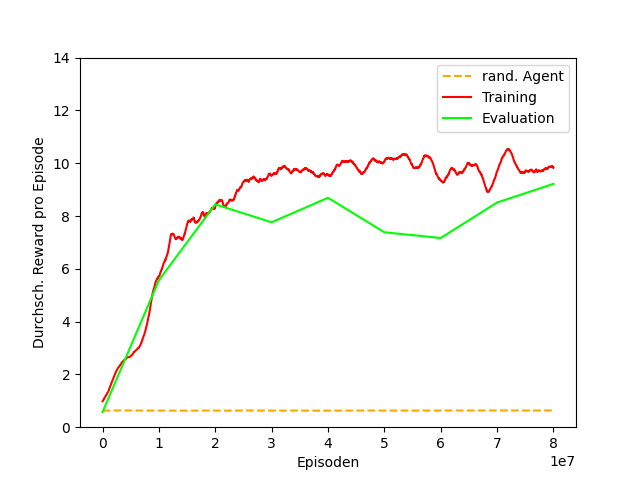
\includegraphics[scale=0.5]{abb/_graphen/floor_80Mio_200lvl_15act_Training_evalAsTraining}
        \caption{Evaluation: one-shot, auf 50 Leveln, 8 Checkpoints des Trainings}
        \label{fig:grph_floor_80Mio_200lvl_15act_Training_1}
    \end{minipage}
    \centering
    \begin{minipage}{0.48\linewidth}
        \centering
        \textbf{Unbeschränkt Level}\par\medskip
        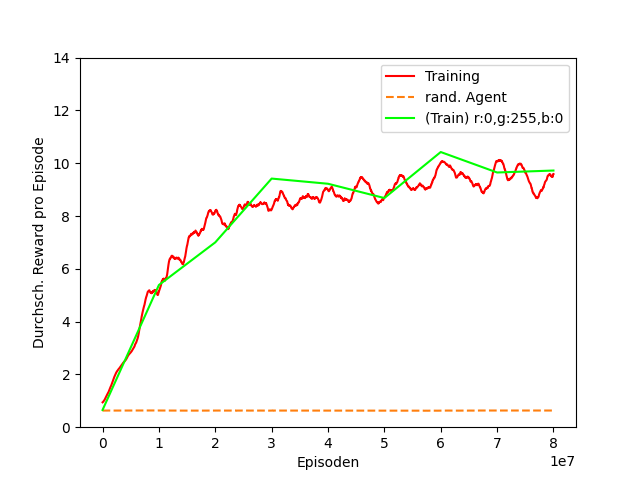
\includegraphics[scale=0.5]{abb/_graphen/floor_80Mio_inflvl_15act_Training_evalAsTraining_14}
        \caption{Evaluation: one-shot, auf 50 Leveln, 8 Checkpoints des Trainings}
        \label{fig:grph_floor_80Mio_inflvl_15act_evalAsTraining}
    \end{minipage}
\end{figure}

\begin{center}
 \begin{table}[htb!]
 \begin{center}
  \begin{tabular}{ l c c c c }
    \hline
		               & Zeitschritte & Anzahl Level & Hintergrund & Farbe Orb \\ \hline \hline
     200 Level           & 80 Mio       & 200		  & 	    normal & r:0, g:255, b:0 \\ \hline
     Unbeschr. Level & 80 Mio       & unbeschr.      & 	    normal & r:0, g:255, b:0 \\ \hline
     Evaluation 		& -	        	   & 1			  & 	    normal 	& r:0, g:255, b:0 \\ \hline
    \hline
  \end{tabular}
  \caption{Übersicht über geltende Rahmenbedingungen in Training und Evaluation - 3.}
  \label{tab:tab_durch_EXP_trainSetting3}
  \end{center}
 \end{table}
\end{center} 

\textbf{Diskussion:} Der direkte Vergleich der beiden Agenten zeigt eindeutig, dass die hohe intrinsische Diversität der Level-Distribution von Procgen \cite{cobbe2019procgen}[S.2] eine große Hilfe beim Erlernen von Generalisierung ist. Die Sample Efficiency ist von der prozeduralen Level-Generierung in diesem Fall weder positiv noch negativ beeinflusst. Das Procgen-Paper zeigt in seinem Experiment \emph{500 Level Generalization} jedoch klar, dass die Auswirkungen der Eigenschaften von Procgen nicht in allen Atari-Environments so drastisch sind (vgl. siehe Abbildung \ref{generalization_500lvl_procgen}). 

Das Spiel Chaser ist durch die Anwesenheit der Orbs eine einfache Umgebung für einen RL-Agenten, welcher auf optischen Inputs beruht. Die Orbs bieten dem Agenten dadurch, dass sie eingesammelt werden können die visuelle Information darüber, wo er schon gewesen ist und wo er noch hin muss. Darüber hinaus geben die Orbs beim einsammeln einen kleinen Reward. Auch wenn der Reward sehr klein ist (0,04 im Vergleich mit 10, implizit für den letzten Orb) leidet dieses Environment nicht unter dem bekannten \emph{Sparse-Reward-Problem}. 

Bei diesem Problem bietet das Environment des Agenten über lange Zeit keinen Reward und er ist darauf angewiesen viele Aktionen auszuführen, bevor überhaupt ein positiver Reward erwartet werden kann. Das Atari-Spiel \dq Montezuma's Revenge\dq{} stellt hierfür ein gutes Beispiel dar. Hier muss der Spieler häufig Schlüssel einsammeln, die zwar den Score erhöhen, jedoch gehören diese Schlüssel oft zu Türen, die mehrere Räume entfernt sein können.

\paragraph{Antwort: Set 1, Punkt 2}
Die zweite Frage des ersten Sets (\ref{lst:itemList_EXP_durch_fragen1}) kann nun vollständig beantwortet werden. Die aus der prozeduralen Level-Generierung resultierende unbeschränkte Anzahl an möglichen Trainings-Leveln bzw. Größe der Trainings-Sets, hilft im Chaser-Environment eindeutig die Generalisierungslücke zu schließen. Jedoch muss das Ergebnis weiter mit größeren Experimenten untersucht werden, bspw. über mehrere Seeds hinweg. Das hier durchgeführte Experiment unterstützt lediglich die Hypothese, dass die intrinsische Diversität ideal für die Evaluation von Generalisierung und Sample Efficiency ist \cite{cobbe2019procgen}[S.9]. 


%################################################################################################################
%################################################################################################################
%FARBÄNDERUNGEN
%################################################################################################################
%##################################################################################################   ##############
\subsection{Visuelle Augmentation - Farbänderungen}\label{absch_EXP_durch_serie1}
Im folgenden Unterkapitel werden Experimente durchgeführt, welche visuelle Änderungen des Trainings- bzw. Evaluations-Environments untersuchen. Die Änderungen des Environments werden in den jeweiligen Experimenten dargelegt.

\subsubsection{Maskierung der Orbs}\label{sub_absch_EXP_durch_serie1_orbsMaskieren}
Wie in Unterkapitel \ref{absch_RL_chaser} erwähnt, ist es das Ziel des Agenten in Chaser alle Orbs einzusammeln. Erst dann gilt eine Episode als erfolgreich abgeschlossen. Dadurch eignen sich die Orbs für Maskierungen und Änderungen ihre Anwesenheit bzw. Erscheinung. Zu diesem Zweck wird im Environment das Hintergrundbild durch eines derselben Größe mit der RGB-Farbe (r:0, g:255, b:0) monoton ersetzt. Die gewählte Farbe entspricht der Farbe der Orbs und maskiert ihre visuelle Anwesenheit. Ein Bild des resultierenden Inputs für den Agenten kann dem Anhang  \ref{anh_env_bilder_chaser} der Abbildung \emph{Hintergrund grün} entnommen werden. Dem Agenten fehlt damit jede visuelle Information der Orbs. Das Reward-System bleibt weiter bestehen. Betritt der Agent ein Feld, welches er zuvor noch nicht besucht hat, bekommt er den Orb-Reward von 0,04. Das aufgeführte Experiment zeigt das Training und die Evaluation eines Agenten, welcher für 5 Mio. Zeitschritte auf einem Level trainiert. Dieses Experiment weicht von der one-shot Evaluation, wie in \ref{subsec_EXP_durch_fragen} definiert ab. Hier ist jeder Checkpoint 50 Mal auf dem einen bekannten Trainings-Level evaluiert.



\begin{figure}[htp!]
   \centering
   \captionsetup{width=0.45\linewidth} 
    \begin{minipage}{0.48\linewidth}
        \centering\
        \textbf{Training - 5 Mio. Zeitschritte}\par\medskip
        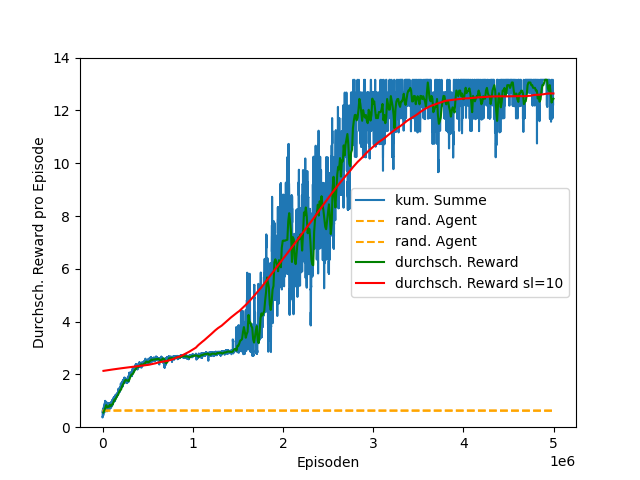
\includegraphics[scale=0.5]{abb/_graphen/green_5Mio_1lvl_15act_Training}
        \caption{Training mit monoton grünem Hintergrund.}
        \label{fig:grph_green_5Mio_1lvl_15act_Training}
    \end{minipage}
    \centering
    \begin{minipage}{0.48\linewidth}
        \centering
        \textbf{Evaluation}\par\medskip
        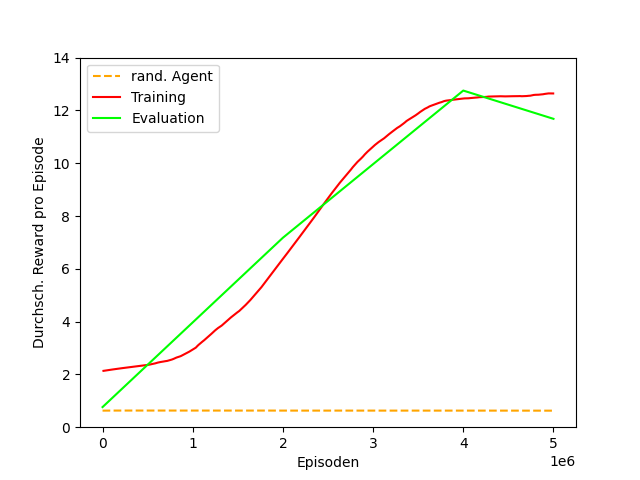
\includegraphics[scale=0.5]{abb/_graphen/green_5Mio_1lvl_15act_Training_evalAsTraining} 
        \caption{Eval: one-shot, auf bekanntem Level.}
        \label{fig:grph_green_5Mio_1lvl_15act_Training_evalAsTraining}
    \end{minipage}
\end{figure}

\begin{center}
%\vskip-0.5cm
 \begin{table}[htb!]
 \begin{center}
  \begin{tabular}{ l c c c c }
    \hline
			       	& Zeitschritte 	& Anzahl Level 	& Hintergrund 	& Farbe Orb \\ \hline \hline
     Level-Anzahl 1     	& 5 Mio       	& 1			& 	     r:0, g:255, g:0	& r:0, g:255, b:0 \\ \hline
     Evaluation 		& - 	           	& 1			& 	    r:0, g:255, g:0 	& r:0, g:255, b:0 \\ \hline
    \hline
  \end{tabular}
  \caption{Übersicht über geltende Rahmenbedingungen in Training und Evaluation - 4.}
  \label{tab:tab_durch_EXP_trainSetting4}
  \end{center}
 \end{table}
\end{center} 

\textbf{Diskussion:} Trotz des grünen Hintergrunds, welcher die visuellen Orb-Informationen maskiert, ist der Agent bereits nach 2,8 Mio. Zeitschritten in der Lage das Level im Training konsistent zu lösen. Auf die Evaluation in ungesehenen Leveln kann hier vorerst verzichtet werden, da in Unterkapitel \ref{par:durch_EXP_vgl_200_1} schon gezeigt wird, dass ein Agent mit einem einzelnen Trainings-Level nicht generalisiert. 
Der Graph von Abbildung \ref{fig:grph_green_5Mio_1lvl_15act_Training_evalAsTraining} zeigt starkes Overfitting auf dem Trainings-Level. Wie dieses Trainingsszenario mit maskierter Orb-Information in größerem Maßstab abläuft, wird im folgenden Paragraphen untersucht.

\paragraph{Vergleich Level-Anzahl: 200, unbeschr., mit grünem Hintergrund}\label{par:durch_EXP_vgl_200_unbeschr_green}
Für das folgende Experiment werden zwei Agenten, einer mit 200 Trainings-Leveln und einer mit unbeschränkter Level-Anzahl, für 80 Mio. Zeitschritte trainiert. Bei diesen Trainings ist der Hintergrund, wie im Paragraphen zuvor, monoton in derselben Farbe wie die Orbs und maskiert deren visuelle Erscheinung. Hierfür werden zwei neue Agenten trainiert.

\begin{figure}[htp!]
   \centering
   \captionsetup{width=0.45\linewidth} 
    \begin{minipage}{0.48\linewidth}
        \centering\
        \textbf{200 Level}\par\medskip
        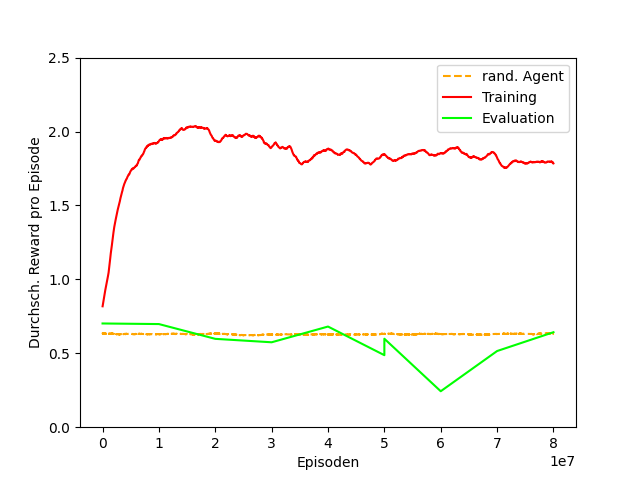
\includegraphics[scale=0.5]{abb/_graphen/green_80Mio_200lvl_15act_Training_evalAsTraining}
        \caption{Training mit grünem Hintergrund in 200 Leveln}
        \label{fig:grph_green_80Mio_200lvl_15act_Training_evalAsTraining_}
    \end{minipage}
    \centering
    \begin{minipage}{0.48\linewidth}
        \centering
        \textbf{Unbeschränkt Level}\par\medskip
        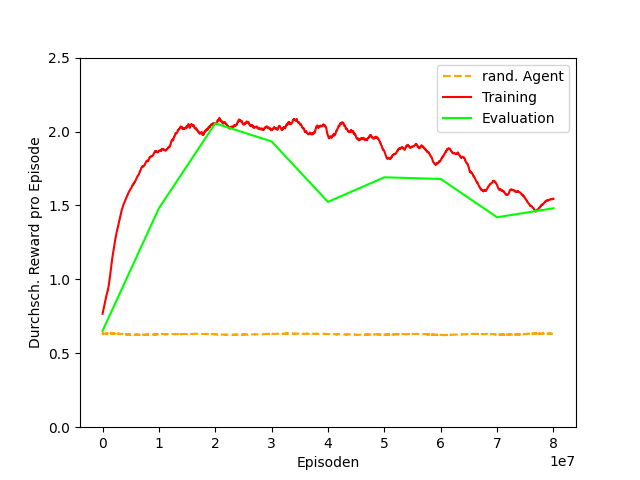
\includegraphics[scale=0.5]{abb/_graphen/green_80Mio_inflvl_15act_Training_evalAsTraining} 
        \caption{Training mit grünem Hintergrund in unbeschr. Leveln}
        \label{fig:grph_green_80Mio_inflvl_15act_Training_evalAsTraining_}
    \end{minipage}
\end{figure}

\begin{center}
%\vskip-0.5cm
 \begin{table}[htb!]
 \begin{center}
  \begin{tabular}{ l c c c c }
    \hline
			       	& Zeitschritte 	& Anzahl Level 	& Hintergrund	 	& Farbe Orb \\ \hline \hline
     200 Level     	& 80 Mio       	& 200		&  r:0, g:255, g:0	& r:0, g:255, b:0 \\ \hline
     Unbeschr. Level   	& 80 Mio       	& unbeschr.	&  r:0, g:255, g:0	& r:0, g:255, b:0 \\ \hline
     Evaluation 		& - 	           	& 50			&  r:0, g:255, g:0 	& r:0, g:255, b:0 \\ \hline
    \hline
  \end{tabular}
  \caption{Übersicht über geltende Rahmenbedingungen in Training und Evaluation - 5.}
  \label{tab:tab_durch_EXP_trainSetting5}
  \end{center}
 \end{table}
\end{center} 

Abbildung \ref{fig:grph_green_80Mio_200lvl_15act_Training_evalAsTraining_} zeigt den Agenten, welcher für 80 Mio. Zeitschritte auf 200 verschiedenen Leveln trainiert wurde. Abbildung \ref{fig:grph_green_80Mio_inflvl_15act_Training_evalAsTraining_} zeigt den Agenten, welcher ebenfalls für 80 Mio. Zeitschritte trainiert wurde, jedoch mit unbeschränkter Level-Anzahl. 

\textbf{Diskussion:} Der Agent mit 200 Leveln im Training zeigt keinerlei Generalisierung. Bei 60 Mio. Zeitschritten lernt der Agent sogar etwas, was ihn schlechter als den zufällig laufenden Agenten macht. Im Kontrast dazu schließt der Agent, welcher mit einer unbeschränkten Level-Anzahl trainiert wurde, die Generalisierungslücke. Vergleicht man hingegen diese beiden Agenten mit den Agenten, welche die Orb-Information während des Trainings haben (\ref{par:durch_EXP_vgl_200_unbeschr}), kristallisiert sich die Hypothese heraus, dass die Orbs eine notwendige visuelle Information darstellen. Beide Agenten mit grünem Hintergrund, egal in wie vielen Leveln sie trainiert wurden, erreichen keine konstanten Siege im Environment. Genauer zeigt die Evaluation, dass keiner der Agenten auch nur ein Level erfolgreich abgeschlossen hat. Diese Ergebnisse werfen die Frage auf, wie ein Agent abschneidet, welcher mit der visuellen Orb-Information trainiert ist, wenn ihm in der Evaluation diese Information entzogen wird. \\


\begin{figure}[htp!]
   \centering
   \captionsetup{width=0.45\linewidth} 
    \begin{minipage}{0.48\linewidth}
        \centering\
        \textbf{Fehlende Orb-Information}\par\medskip
        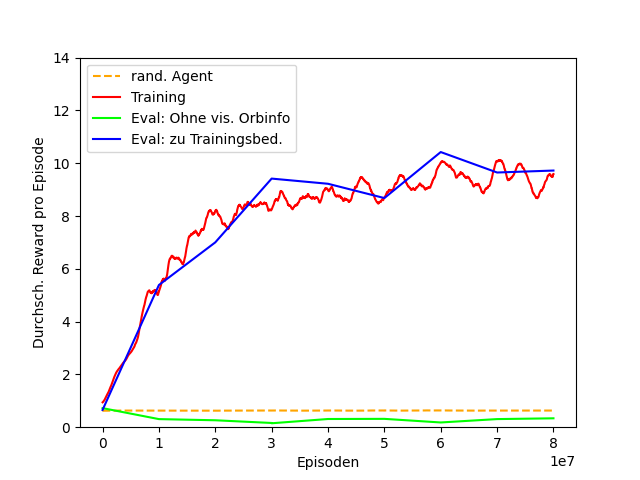
\includegraphics[scale=0.5]{abb/_graphen/floor_80Mio_inflvl_15act_Training_evalAsTraining_evalNoOrb}
        \caption{Evaluation mit und ohne visuelle Orb-Information.}
        \label{fig:floor_80Mio_inflvl_15act_Training_evalAsTraining_evalNoOrb}
    \end{minipage}
\end{figure}

\begin{center}
%\vskip-0.5cm
 \begin{table}[htp!]
 \begin{center}
  \begin{tabular}{ l c c c c }
    \hline
		               & Zeitschritte & Anzahl Level & Hintergrund & Farbe Orb \\ \hline \hline
     Training              & 80 Mio       & unbeschr.	  & 	    normal & r:0, g:255, b:0 \\ \hline
     Eval. wie Training & -              & 50	           & 	    normal & r:0, g:255, b:0 \\ \hline
     Eval. ohne Orbs 	& -	        	   & 50		  & 	    normal 	& vis. nicht vorhanden \\ \hline
    \hline
  \end{tabular}
  \caption{Übersicht über geltende Rahmenbedingungen in Training und Evaluation - 6.}
  \label{tab:tab_durch_EXP_trainSetting6}
  \end{center}
 \end{table}
\end{center} 


%\subsubsection{}

Um die Hypothese zu bestätigen, wird der Agent aus Experiment \ref{par:durch_EXP_vgl_200_unbeschr} mit unbeschränkten Trainings-Leveln wiederverwendet. Dieser Agent weist die beste Generalisierung der bisher trainierten Agenten auf und eignet sich daher am besten für dieses Experiment. Abbildung \ref{fig:floor_80Mio_inflvl_15act_Training_evalAsTraining_evalNoOrb} zeigt die Evaluation mit und ohne visuelle Information der Orbs. Die Agenten sind beide auf denselben Leveln evaluiert. 

\textbf{Diskussion:} Die beiden Graphen zeigen eindeutig, dass die visuelle Information der Orbs unentbehrlich für den Erfolg im gewählten Spiel sind. Beim Start des Trainings zeigt der Agent ohne die visuelle Information (hier grün) noch dieselbe Performance wie der Random-Agent (hier orange-gestrichelt). Bereits beim ersten Checkpoint nach 10 Mio. Zeitschritten im Training, ist seine Performance schlechter als die des Random-Agenten. Die Leistung der anderen Checkpoints oszilliert um einen Wert unterhalb dem des Random-Agenten. 

\paragraph{Antwort: Set 2, Punkt 1}
Nun kann die erste Frage des zweiten Sets (\ref{lst:itemList_EXP_durch_fragen2}) beantwortet werden. Die visuelle Information der Orbs ist notwendig, um unbekannte Level erfolgreich abzuschließen. Es ist egal, ob ein Agent mit dieser Restriktion schon im Training oder erst in der Evaluation konfrontiert wird. Die allgemeine Performance reicht kaum über die eines Random-Agentrn hinaus. Weiter zeigt Abbildung \ref{fig:grph_green_80Mio_inflvl_15act_Training_evalAsTraining_}, dass die Performance der Agenten ab ca. 20 Mio. Zeitschritten sowohl im Trainings, als auch in der Evaluation einen Abwärtstrend aufweist. 


\subsubsection{Farbänderungen der Orbs}\label{sub_absch_EXP_durch_farbÄnderungen}
Im vergangenen Unterkapitel wird gezeigt, dass die visuelle Information der Orbs  ein essenzieller Bestandteil zum erfolgreichen Abschluss unbekannter Level ist. Im folgenden Unterkapitel wird untersucht, welche Auswirkungen farbliche Änderungen der Orbs in der Evaluation auf die Performance eines Agenten haben, der keine dieser Änderungen im Training gesehen hat. Weiter wird hier untersucht, ob eine Konzeptualisierung des Orbs im Training stattfindet. Hierfür wird zunächst wieder der Agent aus Paragraph \ref{par:durch_EXP_vgl_200_unbeschr_green}, mit unbeschränkter Level-Anzahl und normalem Hintergrund, weiteren Evaluationen unterzogen. 


\paragraph{Zufälliger Wert für Grün}\label{par:durch_EXP_farbÄnd_grünZufällig}
Zuerst wird untersucht, wie die Performance in der Evaluation ausfällt, wenn dem Orb in jedem Frame ein neuer Wert für g in RGB, mitgegeben wird. Ein Frame dieser Einstellung kann dem Anhang \ref{anh_env_bilder_chaser} dem Bild \emph{Orb-Farbe: gruen, zufaellig 0-255} entnommen werden. Resultierend aus der Änderung der Orb-Farbe in jedem Frame, flackert jeder Orb in verschiedenen Grüntönen.

\begin{figure}[htp!]
   \centering
   \captionsetup{width=0.45\linewidth} 
    \begin{minipage}{0.48\linewidth}
        \centering\
        \textbf{Zufällige Grüntöne}\par\medskip
        \includegraphics[scale=0.5]{abb/_graphen/floor_80Mio_inflvl_15act_Training_evalRandomGreens}
        \caption{Evaluation mit zufälligen Grüntönen der Orbs}
        \label{fig:floor_80Mio_inflvl_15act_Training_evalRandomGreens}
    \end{minipage}
\end{figure}

\begin{center}
%\vskip-0.5cm
 \begin{table}[htp!]
 \begin{center}
  \begin{tabular}{ l c c c c }
    \hline
		               & Zeitschritte & Anzahl Level & Hintergrund & Farbe Orb \\ \hline \hline
     Training              & 80 Mio       & unbeschr.	  & 	    normal & r:0, g:255, b:0 \\ \hline
     Eval. zufälliges Grün 	& -	        	   & 50		  & 	    normal 	& r:0, g:0-255, b:0 \\ \hline
     Eval. zufälliges Grün 	& -	        	   & 50		  & 	    normal 	& r:0, g:1-255, b:0 \\ \hline
    \hline
  \end{tabular}
  \caption{Übersicht über geltende Rahmenbedingungen in Training und Evaluation - 7.}
  \label{tab:tab_durch_EXP_trainSetting7}
  \end{center}
 \end{table}
\end{center} 

Der blaue Graph zeigt die Evaluation mit einem zufälligen Grünton, ohne die Option auf schwarze Orbs - der rote Graph zeigt die Evaluation mit der Option auf schwarze Orbs. 

\textbf{Diskussion:} Die Auswertung dieser Daten legt vorerst nahe, dass keine Konzeptualisierung des Orbs stattfindet und dennoch ist der Agent bei den Checkpoints ab 60 Mio. Zeitschritte deutlich besser, als der Random-Agent. Hier muss erwähnt werden, dass die Zuweisung einer neuen, zufälligen Orb-Farbe in jedem Frame eine starke Änderung der gewohnten Pixel-Verteilung darstellt. So zeigt der Agent in beiden Evaluationen keine befriedigende Generalisierung für diese Änderungen auf. Motiviert durch dieses Experiment wird im folgenden Paragraphen untersucht, wie sich eine statische Änderung des Grün-Anteils auf die Performance auswirkt.

\paragraph{Grünabstufungen in 50er Schritten}\label{par:durch_EXP_farbÄnd_grünAbstufung}
Zur Erinnerung, die Farbe der Orbs im Training hat die RGB-Werte (r:0, g:255, b:0). Hier wird in jeder Evaluation der grün-Wert (G-Wert) um 50 verringert, angefangen bei 250 bis 0. Die Graphen der Abbildung, außer dem Trainingsgraphen, haben alle die jeweilige Farbe, die in der Evaluation verwendet wurde.

\begin{figure}[htp!]
   \centering
   \captionsetup{width=0.45\linewidth} 
    \begin{minipage}{0.48\linewidth}
        \centering\
        \textbf{50er Grüntöne - 1}\par\medskip
        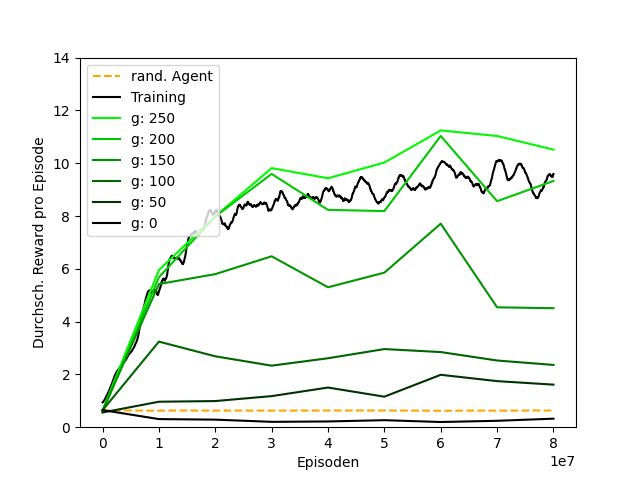
\includegraphics[scale=0.5]{abb/_graphen/floor_80mio_inflvl_Training_eval50Green}
        \caption{Evaluation von Grüntönen, schwärzer werdend.}
        \label{fig:floor_80Mio_inflvl_15act_Training_eval50Green}
    \end{minipage}
\end{figure}
\begin{center}
 \begin{table}[htp!]
 \begin{center}
  \begin{tabular}{ l c c c c }
    \hline
		               & Zeitschritte & Anzahl Level & Hintergrund & Farbe Orb \\ \hline \hline
     Training              & 80 Mio       & unbeschr.	  & 	    normal & r:0, g:255, b:0 \\ \hline
     Eval. Grün: 250 	& -	        	   & 50		  & 	    normal 	& r:0, g:250, b:0 \\ \hline
     Eval. Grün: 200 	& -	        	   & 50		  & 	    normal 	& r:0, g:200, b:0 \\ \hline
     Eval. Grün: 150 	& -	        	   & 50		  & 	    normal 	& r:0, g:150, b:0 \\ \hline
     Eval. Grün: 100 	& -	        	   & 50		  & 	    normal 	& r:0, g:100, b:0 \\ \hline
     Eval. Grün: 50 	& -	        	   & 50		  & 	    normal 	& r:0, g:50, b:0 \\ \hline
     Eval. Grün: 0 	& -	        	   & 50		  & 	    normal 	& r:0, g:0, b:0 \\ \hline
    \hline
  \end{tabular}
  \caption{Übersicht über geltende Rahmenbedingungen in Training und Evaluation - 8.}
  \label{tab:tab_durch_EXP_trainSetting8}
  \end{center}
 \end{table}
\end{center} 

\textbf{Diskussion:} Die Auswertung der Abbildung \ref{fig:floor_80Mio_inflvl_15act_Training_eval50Green} zeigt eine interessante These. Die Ergebnisse zeigen, dass die Performance stetig abnimmt, solange der G-Wert weiter abnimmt. Mit jeder weiteren Evaluation wird die Generalisierungslücke größer. So weisen die beiden Graphen mit einem G-Wert von $200$ und $250$ fast gleich gute Performance und nahezu keine Probleme bei der Generalisierung auf. Wohingegen der Graph mit einem G-Wert von $150$ kaum besser als halb so gut ist, wie die zwei Graphen zuvor. Die restlichen drei Graphen mit den G-Werten $100$, $50$ und $0$ zeigen einen stetigen Abstieg der Performance in der Evaluation. Bei einem G-Wert von 0 ist der Agent sogar schlechter als der Random-Agent.

Um die These weiter zu untersuchen, wird folgend ein ähnliches Experiment vorgestellt, in dem der G-Wert konstant bei $255$ ist und sich die Werte für rot und blau von Evaluation zu Evaluation verändern. Zuvor wurden die Orbs dunkler und dunkler, bis hin zu schwarz - folgend werden die Orbs immer heller, bis hin zu weiß. Wie zuvor haben die Graphen der Abbildung \ref{fig:floor_80Mio_inflvl_15act_Training_eval50Others} die Orb-Farbe der jeweiligen Evaluation. Die Farbe Weiß wird hier aus Gründen der Sichtbarkeit in Grau dargestellt.  \newline

\begin{figure}[htp!]
   \centering
   \captionsetup{width=0.45\linewidth} 
    \begin{minipage}{0.48\linewidth}
        \centering\
        \textbf{50er Grüntöne - 2}\par\medskip
        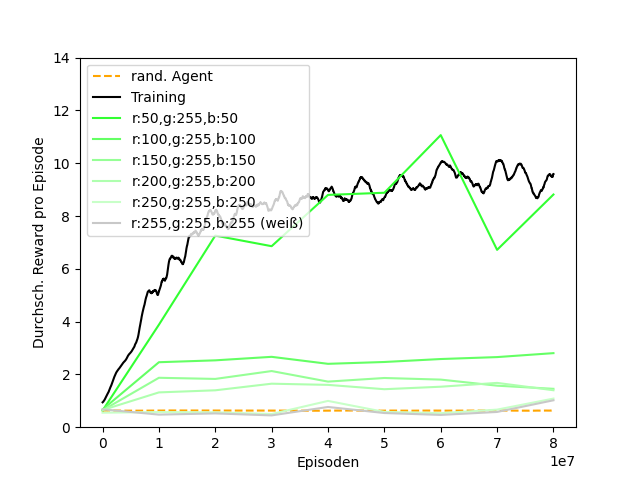
\includegraphics[scale=0.5]{abb/_graphen/floor_80mio_inflvl_Training_eval50Others}
        \caption{Evaluation von Grüntönen, weißer werdend.}
        \label{fig:floor_80Mio_inflvl_15act_Training_eval50Others}
    \end{minipage}
\end{figure}
\begin{center}
 \begin{table}[htp!]
 \begin{center}
  \begin{tabular}{ l c c c c }
    \hline
		               			& Zeitschritte & Anzahl Level & 		Hintergrund & Farbe Orb \\ \hline \hline
     Training              			& 80 Mio       & unbeschr.	  & 	    		normal & r:0, g:255, b:0 \\ \hline
     Eval. r:50, b:50	 	& -	        	   & 50		  	  &			normal & r:50, g:255, b:50 \\ \hline
     Eval. r:100, b:100	& -	        	   & 50		  & 	    				normal & r:100, g:255, b:100  \\ \hline
     Eval. r:150, b:150 	& -	        	   & 50		  & 	    			normal & r:150, g:255, b:150  \\ \hline
     Eval. r:200, b:200 	& -	        	   & 50		  & 	    			normal & r:200, g:255, b:200 \\ \hline
     Eval. r:250, b:250 	& -	        	   & 50		  & 	    			normal & r:250, g:255, b:250 \\ \hline
     Eval. r:255, b:255 	& -	        	   & 50		  & 	    			normal & r:255, g:255, b:255 \\ \hline
    \hline   
  \end{tabular}
  \caption{Übersicht über geltende Rahmenbedingungen in Training und Evaluation - 9.}
  \label{tab:tab_durch_EXP_trainSetting9}
  \end{center}
 \end{table}
\end{center} 

\textbf{Diskussion:} Die Auswertung der Abbildung \ref{fig:floor_80Mio_inflvl_15act_Training_eval50Others} liefert Ergebnisse, welche die zuvor aufgestellte These vorerst widerlegen. Verglichen mit Abbildung \ref{fig:floor_80Mio_inflvl_15act_Training_eval50Green} zeigt Abbildung \ref{fig:floor_80Mio_inflvl_15act_Training_eval50Others} keinen stetigen Abstieg der Performance mit fortlaufender Evaluation. Stattdessen schneiden die Evaluationen mit R- und B-Werten $100$ bis $255$ deutlich schlechter ab, als die Evaluation mit schwärzer werdenden Orbs. Darüber hinaus zeigen die Graphen mit den R- und B-Werten (R-Werte, B-Werte) $100$ bis $250$ eine deutlich geringere Varianz, als die korrespondierenden Graphen der Abbildung \ref{fig:floor_80Mio_inflvl_15act_Training_eval50Green}. Eine mögliche Erklärung für die generell schlechtere Leistung der Graphen mit R- und B-Werten von $100$ bis $250$ kann sein, dass die Abweichung der Orb-Farbe, verglichen zur Farbe im Training, an zwei Farbwerten der RGB-Farbe verändert wurde. Dementgegen wurde in der Evaluation von Abbildung \ref{fig:floor_80Mio_inflvl_15act_Training_eval50Green} jeweils nur der G-Wert verändert. 

Die Veränderung an zwei Stellschrauben der RGB-Farbe stellt im Kontext des gesamten Bildes eine größere Veränderung der Pixel-Verteilung dar. Aus beiden Experimenten dieses Paragraphen geht hervor, dass jene Durchläufe, bei denen die Abweichung der farblichen Distanz zu einem Input-Frame vom Training zu stark sind, generell schlecht abscheiden. So stellt eine Veränderung der Orbs um jeweils 50 in den R- und B-Werten (100 gesamt) keine Herausforderung für den Agenten aus Abbildung \ref{fig:floor_80Mio_inflvl_15act_Training_eval50Others} dar. Dagegen hat eine Änderung um 105 am G-Wert, verglichen mit dem Trainingszustand des Orbs, deutlich gravierendere Auswirkungen auf die Performance (siehe Abbildung \ref{fig:floor_80Mio_inflvl_15act_Training_eval50Green}).  
Das bestätigt die intuitive These, dass Änderungen an zwei der drei Pixel-Werte und die daraus resultierende Änderung der Pixel-Verteilung größere Auswirkungen auf die Performance hat, als Änderungen an nur einem der Werte. Weiter lässt sich aus den Ergebnissen schließen, dass der Agent stark auf die Farbe des Orbs overfitted. Diese These wird im folgenden Paragraphen genauer untersucht. 


\paragraph{Experimente mit verschiedenen Orb-Farben}
\label{par:durch_EXP_farbÄnd_rgbOrbfarben}

Für die folgenden Experimente werden zwei weitere Agenten trainiert. Einer mit roten und einer mit blauen Orbs (\emph{Agent-Rot} und \emph{Agent-Blau}), beide mit dem normalen Hintergrund. Bilder des jeweiligen Inputs der Agenten können dem Anhang entnommen werden (\ref{anh_env_bilder_chaser}, Titel: \emph{Blaue Orbs}, \emph{Rote Orbs}). Beide neuen Agenten sind für eine Dauer von 80 Mio. Zeitschritten und mit einer unbeschränkten Anzahl an Leveln trainiert. Die Agenten unterscheiden sich somit lediglich in der Farbe, welche die Orbs während des Trainings haben. 

In dieser Reihe von Experimenten werden die oben beschrieben Agenten, mit dem in Unterkapitel \ref{sec:absch_EXP_durch_reproduktion} vorgestellten Agenten mit normalem Hintergrund und grünen Orbs (\emph{Agent-Grün}) verglichen. Dieser Agent dient hier als Baseline für den Vergleich der Agenten. In der Evaluation wird jeder Agent zum Vergleich mit seiner Orb-Farbe wie im Training und den Trainingsfarben der beiden anderen Agenten konfrontiert. Alle Agenten haben den jeweiligen Farb-Channel auf 255 und die anderen beiden auf 0 gesetzt. So entspricht die Farbe Rot dem RGB-Wert $ r:255, g=0, b=0 $, die anderen Farben ergeben sich analog. Somit weisen die drei Orb-Farben eine farbliche Distanz von $510$ auf.

\begin{figure}[htp!]
   \centering
   \captionsetup{width=0.48\linewidth} 
    \begin{minipage}{0.48\linewidth}
        \centering\
        %\medskip
        \textbf{Training - Rot}\par
        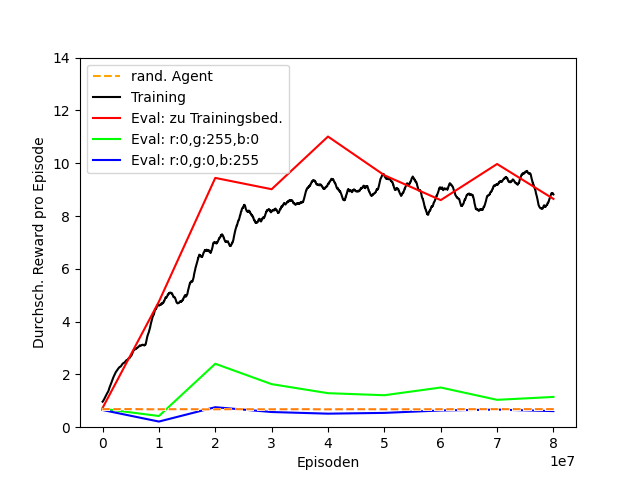
\includegraphics[scale=.358]{abb/_graphen/floor_80Mio_inflvl_15_act_TrainingRot_evalRGB}
        \caption{Training mit rotem Orb und normalem Hintergrund.}
        \label{fig:grph_red_80Mio_200lvl_15act_Training_evalAsTraining}
    \end{minipage}
    \centering
    \begin{minipage}{0.48\linewidth}
        \centering
        \textbf{Training - Grün}\par%\medskip 
        %0,49
        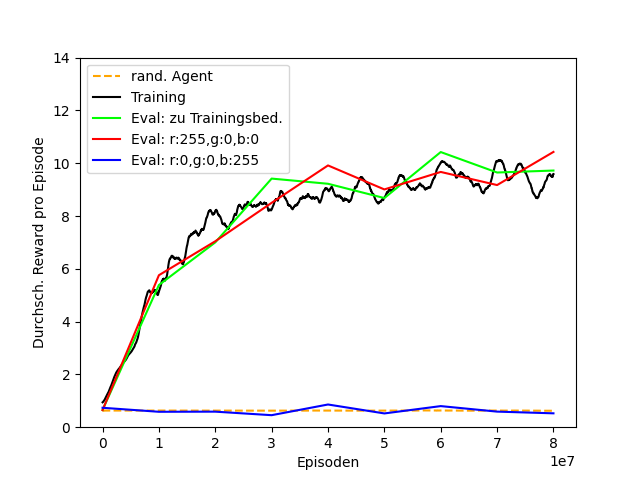
\includegraphics[scale=0.515]{abb/_graphen/floor_80Mio_inflvl_15_act_TrainingGreen_evalRGB} 
        \caption{Training mit grünem Orb und normalem Hintergrund.}
        \label{fig:grph_green_80Mio_inflvl_15act_Training_evalAsTraining}
    \end{minipage}
    \centering
    \begin{minipage}{0.48\linewidth}
    	\centering
        \textbf{Training - Blau}\par%\medskip
        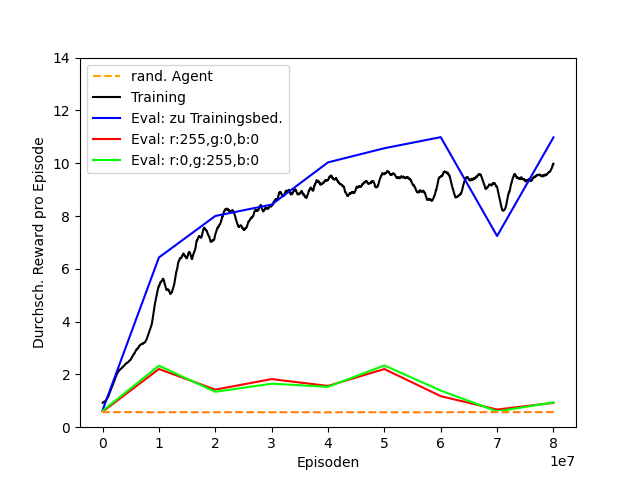
\includegraphics[scale=0.358]{abb/_graphen/floor_80Mio_inflvl_15_act_TrainingBlau_evalRGB} 
        \caption{Training mit blauem Orb und normalem Hintergrund.}
        \label{fig:grph_blue_80Mio_inflvl_15act_Training_evalAsTraining}
    \end{minipage}
\end{figure}

\begin{center}
 \begin{table}[htp!]
 \begin{center}
  \begin{tabular}{ l c c c c }
    \hline
		               			& Zeitschritte & Anzahl Level & 		Hintergrund & Farbe Orb \\ \hline \hline
     Training rot              			& 80 Mio       & unbeschr.	  & 	    		normal & r:255, g:0, b:0 \\ \hline
     Training grün              			& 80 Mio       & unbeschr.	  & 	    		normal & r:0, g:255, b:0 \\ \hline
     Training blau             			& 80 Mio       & unbeschr.	  & 	    		normal & r:0, g:0, b:255 \\ \hline
     Eval. rot	 	& -	        	   & 50		  	  &			normal & r:255, g:0, b:50 \\ \hline
     Eval. grün	& -	        	   & 50		  & 	    				normal & r:0, g:255, b:0  \\ \hline
     Eval. blau 	& -	        	   & 50		  & 	    			normal & r:0, g:0, b:255  \\ \hline
    \hline
  \end{tabular}
  \caption{Übersicht über geltende Rahmenbedingungen in Training und Evaluation - 10.}
  \label{tab:tab_durch_EXP_trainSetting10}
  \end{center}
 \end{table}
\end{center} 

\textbf{Diskussion:} Im Training zeigen die unterschiedlichen Agenten sehr ähnliche Leistungen. Keiner der trainierten Agent weist eine relevante Generalisierungslücke auf. Die Abweichungen von der Baseline Agent-Grün ist im Rahmen der erwarteten Varianz, bei der Verwendung tiefer NNs. Wie zu erwarten, ist eine Änderung der Orb-Farbe während der Evaluation eine unüberwindbare Hürde für die Agenten. Dies gilt jedoch nicht für den Agent-Grün. Dieser Agent ist in der Lage mit der unbekannten Orb-Farbe Rot, eine nahezu identische Performance während der Evaluation zu erreichen. Die Evaluationen mit unbekannten Orb-Farben der Agenten Agent-Rot und Agent-Blau ist zwar weit unter der Performance der Evaluation zu Trainingsbedingungen, dennoch sind die beiden Agenten in drei von vier Fällen besser, als der Random-Agent. In Abbildung \ref{fig:grph_red_80Mio_200lvl_15act_Training_evalAsTraining} (Agent-Rot) weist der Graph, welcher die Evaluation mit einem grünen Orb zeigt, eine deutliche Abweichung vom Random-Agenten auf. Die Abweichung wird in Abbildung \ref{fig:grph_blue_80Mio_inflvl_15act_Training_evalAsTraining} noch deutlicher. Hier ist der Agent-Blau in der Lage, mit beiden unbekannten Orb-Farben (hier rot und grün) eine noch deutlichere Abweichung zum Random-Agenten aufzuweisen. Genauer performt der Agent-Blau mit beiden unbekannten Farben nahezu gleich gut. Der Einsturz der Leistung beim Checkpoint 70 Mio. Zeitschritte spiegelt sich ebenso in der Evaluation mit der bekannten Orb-Farbe wieder und ist über ein schlechtes Update der Policy zu erklären. 

In diesem Experiment werden zwar die Orb-Farben in die drei Extreme verändert (siehe Tabelle \ref{tab:tab_durch_EXP_trainSetting10}), jedoch ist der Hintergrund weiterhin ein farbiges Bild mit Textur (siehe Abbildung \ref{fig:pic_chaserGros}). Da die jeweiligen Farben der Orbs einen Farbkanal auf $255$ und die anderen beiden auf $0$ haben, stellen diese Farben die Grundfarbtöne von RBG dar. Um eine der drei Farben weiß zu machen, müssen die beiden Farbkanäle, welche auf $0$ sind, ebenfalls auf $255$ gesetzt werden. Somit weisen alle drei Orb-Farben eine farbliche Distanz zur Farbe Weiß von $510$ RGB-Werten auf.

Um die Unterschiede in der farblichen Distanz der jeweiligen Orb-Farben zum Hintergrund auszuschließen, wird das hier aufgeführte Experiment mit einem weißen Hintergrund wiederholt. 


\paragraph{Experimente mit weißem Hintergrund}\label{par:durch_EXP_farbÄnd_weisserHintergrund}

Im folgenden Paragraphen wird das Experiment der vorangegangenen Paragraphen mit einem weißen Hintergrund wiederholt. Dies soll Unterschiede der jeweiligen Orb-Farbe zum Hintergrund bezüglich Kontrast ausschließen und stellt sicher, dass die Farben alle die selbe farbliche Distanz zum Hintergrund haben. Hierfür werden drei neue Agenten, mit der eben erwähnten Veränderung zu den selben Bedingungen, wie im vorherigen Experiment trainiert. 

Wie zuvor bezeichnet \emph{Agent-Rot} den Agenten welcher mit einem roten Orb trainiert wird. \emph{Agent-Grün} bezeichnet den Agenten mit grünen und \emph{Agent-Blau} den mit blauen Orbs im Training. Ein Bild des aktuellen Agenten-Inputs kann dem Anhang den Bildern mit dem Titel \emph{BG: weiß} entnommen werden (\ref{anh_env_bilder_chaser}).

\begin{figure}[htp!]
   \centering
   \captionsetup{width=0.48\linewidth} 
    \begin{minipage}{0.48\linewidth}
        \centering\
        %\medskip
        \textbf{Training - Rot}\par
        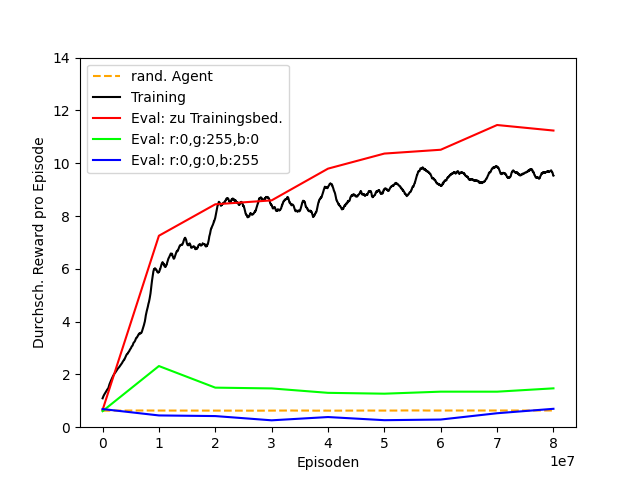
\includegraphics[scale=.5]{abb/_graphen/floor_80Mio_inflvl_15_act_TrainingRot_evalRGB_white}
        \caption{Training mit rotem Orb und weißem Hintergrund.}
        \label{fig:grph_red_80Mio_200lvl_15act_Training_evalAsTraining_white}
    \end{minipage}
    \centering
    \begin{minipage}{0.48\linewidth}
        \centering
        \textbf{Training - Grün}\par%\medskip 
        %0,49
        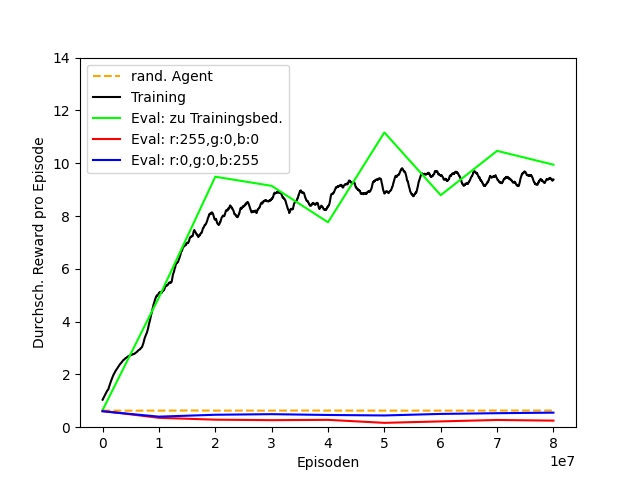
\includegraphics[scale=0.5]{abb/_graphen/floor_80Mio_inflvl_15_act_TrainingGreen_evalRGB_white} 
        \caption{Training mit grünem Orb und weißem Hintergrund.}
        \label{fig:grph_green_80Mio_inflvl_15act_Training_evalAsTraining_white}
    \end{minipage}
    \centering
    \begin{minipage}{0.48\linewidth}
\vspace*{0.5cm}
    	\centering
        \textbf{Training - Blau}\par%\medskip
        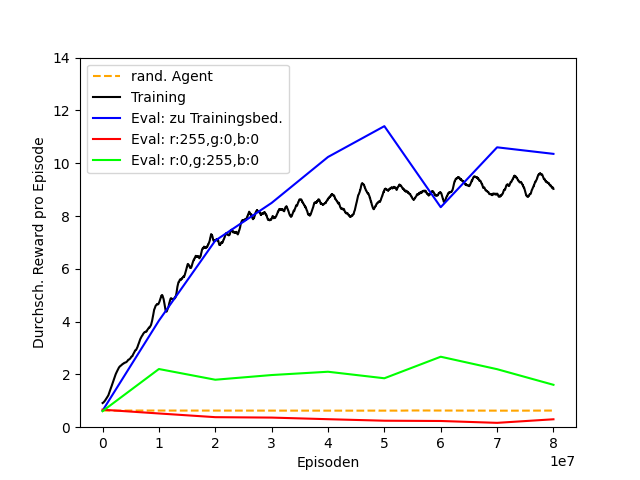
\includegraphics[scale=0.5]{abb/_graphen/floor_80Mio_inflvl_15_act_TrainingBlau_evalRGB_white} 
        \caption{Training mit blauem Orb und weißem Hintergrund.}
        \label{fig:grph_blue_80Mio_inflvl_15act_Training_evalAsTraining_white}
    \end{minipage}
\end{figure}
\begin{center}
 \begin{table}[htp!]
 \begin{center}
  \begin{tabular}{ l c c c c }
    \hline
		               			& Zeitschritte & Anzahl Level & 		Hintergrund & Farbe Orb \\ \hline \hline
     Training rot              			& 80 Mio       & unbeschr.	  & 	    		weiß & r:255, g:0, b:0 \\ \hline
     Training grün              			& 80 Mio       & unbeschr.	  & 	    		weiß & r:0, g:255, b:0 \\ \hline
     Training blau             			& 80 Mio       & unbeschr.	  & 	    		weiß & r:0, g:0, b:255 \\ \hline
     Eval. rot	 	& -	        	   & 50		  	  &			weiß & r:255, g:0, b:50 \\ \hline
     Eval. grün	& -	        	   & 50		  & 	    				weiß & r:0, g:255, b:0  \\ \hline
     Eval. blau 	& -	        	   & 50		  & 	    			weiß & r:0, g:0, b:255  \\ \hline
    \hline
  \end{tabular}
  \caption{Übersicht über geltende Rahmenbedingungen in Training und Evaluation - 11.}
  \label{tab:tab_durch_EXP_trainSetting10}
  \end{center}
 \end{table}
\end{center} 


\textbf{Diskussion:} Wie im oben aufgeführten Experiment, zeigen die Abbildungen \ref{fig:grph_red_80Mio_200lvl_15act_Training_evalAsTraining_white}, \ref{fig:grph_green_80Mio_inflvl_15act_Training_evalAsTraining_white} und \ref{fig:grph_blue_80Mio_inflvl_15act_Training_evalAsTraining_white}, dass die Evaluationen zu Trainingsbedingungen nahezu keine Generalisierungslücke aufweist. Weiter ist Agent-Grün nicht mehr in der Lage, mit den roten Orbs genauso hohe Rewards, wie mit den bekannten grünen Orbs zu erzielen, wie im Experiment zuvor. Hier ist sogar das Gegenteil der Fall. Der Graph der Evaluation mit rotem Orb (\ref{fig:grph_green_80Mio_inflvl_15act_Training_evalAsTraining_white}) ist über jeden Checkpoint hinweg unter dem des Random-Agenten und auch unter dem Graphen der Evaluation mit blauem Orb. Darüber hinaus sind nicht mehr drei von vier Graphen (unterschiedlicher Farben) der Agenten aus den Abbildungen \ref{fig:grph_red_80Mio_200lvl_15act_Training_evalAsTraining_white} und \ref{fig:grph_blue_80Mio_inflvl_15act_Training_evalAsTraining_white} besser als der Random-Agent. Lediglich die Graphen der jeweiligen Evaluation mit grünen Orbs sind besser als der Random-Agent. \\

\paragraph{Antwort: Set 2, Punkt 2}
Die zwei Fragen des zweiten Punkts vom Set zur farblichen Änderung (\ref{par_EXP_durch_fragen2}) sind mit den durchgeführten Experimenten nicht mit ausreichender Sicherheit zu beantworten. Die erste Frage kann klar beantwortet werden. Über das Training mit den geltenden Bedingungen findet keine Konzeptualisierung eines Orbs bezogen auf farbliche Änderungen statt. Die vier Experimente in Unterkapitel \ref{sub_absch_EXP_durch_farbÄnderungen} belegen empirisch, dass jede Veränderung der visuellen Darstellung des Orbs drastische Auswirkungen auf den erhaltenen Reward des Agenten haben. 

Die zweite Frage kann zwar  beantwortet werden, jedoch widersprechen die Ergebnisse der initialen Intuition und werfen wiederum selbst neue Fragen auf. Die beschriebenen Experimente bestätigen, dass sich farbliche Änderungen, nahezu jeder farblichen Distanz, negativ auswirken. Allerdings kann der Agent sein Wissen in diesem einen Fall abstrahieren. So ist der Agent aus Abbildung \ref{fig:grph_green_80Mio_inflvl_15act_Training_evalAsTraining} in der Lage, mit der unbekannten Orb-Farbe Rot, nahezu identische Rewards zu erzielen, wie in der Evaluation zu Trainingsbedingungen mit grünem Orb. Ein blauer Orb hingegen, welcher dieselbe farbliche Distanz zu einem grünen Orb hat, bricht die Generalisierung des Agenten in ungesehenen Leveln. 



\subsubsection{Untersuchung des Speichervermögens}

\paragraph{Experiment zum Speichervermögen}\label{par:durch_EXP_farbÄnd_Speichervermögen}
Folgend wird untersucht, wie viele Level ein Agent innerhalb einer begrenzten Anzahl an Zeitschritten auswendig lernen kann. Das Experiment im Anhang \ref{anh_exp_5mio} zeigt, dass ein Agent im Training bereits nach ca. 1,2 Mio. Zeitschritten in einem Level einen Reward von $ \geq 10$ erreicht. Somit overfitted der Agent bereits nach 1,2 Mio. Zeitschritten stark auf das Trainings-Level. Das Experiment mit grünem Hintergrund zu denselben Trainingsbedingungen zeigt, dass das Level nach circa 2,6 Mio. Zeitschritten ebenso problemlos bestanden werden kann, auch ohne die visuelle Information der Orbs. Diese Ergebnisse motivieren die folgenden Experimente.

Dieses Experiment untersucht mit 30 Agenten, wie viele Level ein Agent im Training innerhalb von 5 Mio. Zeitschritten auswendig lernen kann. Es wird nicht dieselbe one-shot Evaluation wie zuvor angewandt. Dieses Mal wird nach jeder Episode, eines der Trainings-Level, zufällig ausgewählt und das über 50 Iterationen hinweg. Die 30 Agenten sind in zwei Sets mit je 15 Agenten aufgeteilt. Das eine Set trainiert mit dem normalen und das andere mit dem grünem Hintergrund und somit mit maskierter, visueller Orb-Information. Der erste Agent eines Sets trainiert in einem Level, der zweite in zwei usw. Der letzte trainiert in 15 Leveln. Egal in wie vielen Leveln trainiert wird, dem Agenten stehen nur die 5 Mio. Zeitschritte zur Verfügung. Die ersten Balken von links der Abbildungen \ref{fig:grph_floor_80Mio_200lvl_15act_Training_evalAsTraining_1to15} und \ref{fig:grph_green_80Mio_inflvl_15act_Training_evalAsTraining_1to15} repräsentiert den ersten Agenten eines Sets, der Balken ganz rechts den letzten. Jeder Balken ist in vier Abschnitte unterteilt. Der unterste Teil zeigt den ersten Checkpoint (hier rot) nach dem ersten Zeitschritt und zeigt somit ebenso einen Random-Agenten. Checkpoint 2 (hier grün) den Agenten nach 2 Mio. Zeitschritten und Checkpoint 3 (hier blau) nach 4 Mio. Zeitschritten. Der letzte (hier cyan) zeigt die abschließende Evaluation nach 5 Mio. Zeitschritten. Der Anhang bietet eine tabellarische Übersicht über die Erfolgsraten der jeweiligen Agenten (\ref{anh_exp_erfolgsrate}). 

\begin{figure}[htp!]
   \centering
   \captionsetup{width=0.45\linewidth} 
    \begin{minipage}{0.48\linewidth}
        \centering\
        \textbf{Normaler Hintergrund\\0 bis 15 Level}\par\medskip
        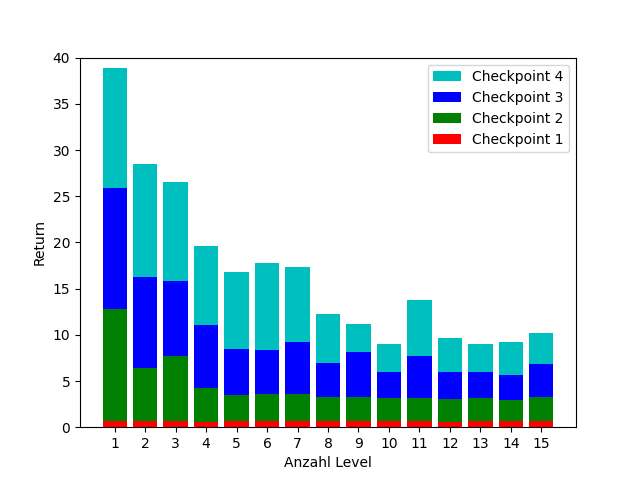
\includegraphics[scale=0.5]{abb/_graphen/serie_auswendig_floor}
        \caption{Training in 1 - 15 Leveln mit normalem Hintergrund.}
        \label{fig:grph_floor_80Mio_200lvl_15act_Training_evalAsTraining_1to15}
    \end{minipage}
    \centering
    \begin{minipage}{0.48\linewidth}
        \centering
        \textbf{Grüner Hintergrund\\0 bis 15 Level}\par\medskip
        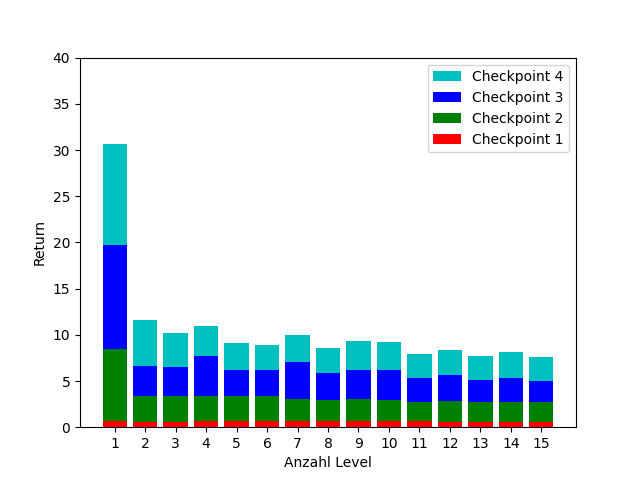
\includegraphics[scale=0.5]{abb/_graphen/serie_auswendig_green} 
        \caption{Training in 1 - 15 Leveln mit grünem Hintergrund.}
        \label{fig:grph_green_80Mio_inflvl_15act_Training_evalAsTraining_1to15}
    \end{minipage}
\end{figure}

\begin{center}
%\vskip-0.5cm
 \begin{table}[htb!]
 \begin{center}
  \begin{tabular}{ l c c c c }
    \hline
			       				& Zeitschritte 	& Anzahl Level 	& Hintergrund	 	& Farbe Orb \\ \hline \hline
     Train. normaler BG  	& 5 Mio       	& 1 - 15		&  normal			& r:0, g:255, b:0 \\ \hline
     Train. grüner BG   	& 5 Mio       	& 1 - 15 		&  r:0, g:255, g:0	& r:0, g:255, b:0 \\ \hline
     Eval. normaler BG 	& - 	           	& 1 - 15			&  normal		 	& r:0, g:255, b:0 \\ \hline
     Eval. grünem BG 	& - 	           	& 1 - 15			&  r:0, g:255, g:0 	& r:0, g:255, b:0 \\ \hline
    \hline
  \end{tabular}
  \caption{Übersicht über geltende Rahmenbedingungen in Training und Evaluation - 12.}
  \label{tab:tab_durch_EXP_trainSetting5}
  \end{center}
 \end{table}
\end{center} 

\textbf{Diskussion:} Der erste Agent von Abbildung \ref{fig:grph_floor_80Mio_200lvl_15act_Training_evalAsTraining_1to15} im direkten Vergleich mit dem ersten Agenten der Abbildung \ref{fig:grph_green_80Mio_inflvl_15act_Training_evalAsTraining_1to15} zeigt einerseits, dass die Performance der jeweiligen Checkpoints mit der visuellen Orb-Information höher ist, was auf eine bessere Sample Efficiency schließen lässt. Andererseits ist der gesamte erhaltene Reward jedes Checkpoints deutlich höher, als der des Agenten mit grünem Hintergrund. Die visuelle Anwesenheit der Orbs verhilft einem Agent also nicht nur zu verbesserter Sample Efficiency, sondern verhilft ihm auch zu einer robusteren Policy. Das lässt sich dadurch erklären, dass die Orbs, sofern sichtbar, eingesammelt werden können und nicht mehr vorhanden sind, sobald sie einmal eingesammelt sind. Das kann dem Agenten helfen eine zielführendere Strategie zu wählen. Das funktioniert jedoch nur unter der Prämisse, dass der Agent eine Vorstellung des finalen Ziels des Environments hat. Die Agenten zwei bis neun der linken Abbildung unterscheiden sich stark von denen der rechten. Die Agenten mit visueller Orb-Information sind in der Lage, bis zu drei Level innerhalb der 5 Mio. Zeitschritte auswendig zu lernen. Der Reward des vierten Checkpoints des dritten Agenten von Abbildung \ref{fig:grph_floor_80Mio_200lvl_15act_Training_evalAsTraining_1to15} liegt bei $10,71$. Dieser Agent schafft 76\% der 50 Wiederholungen seiner Trainings-Level. Im Vergleich hierzu schafft der vierte Checkpoint des ersten Agent aus Abbildung \ref{fig:grph_green_80Mio_inflvl_15act_Training_evalAsTraining_1to15} 78\% dieser Wiederholungen. Der dritte Agent derselben Abbildung schafft lediglich 8\% der Level. Der direkte Vergleich der dritten Agenten der beiden Abbildungen legt nahe, dass die visuelle Information der Orbs ein wichtiger Faktor für den erfolgreichen Abschluss unbekannter Level ist. Hier ergibt sich eine Differenz der Erfolgsrate von 68\%. Diese Ergebnisse unterstützen die des Experiments zur ersten Frage des zweiten Sets. Die Evaluation der letzten vier Agenten der beiden Sets legt nahe, dass die Performance des Agenten mit der visuellen Orb-Information weiter abnehmen wird, bis auf das Niveau der letzten Agenten aus Abbildung \ref{fig:grph_green_80Mio_inflvl_15act_Training_evalAsTraining_1to15}.\\

\paragraph{Antwort: Set 2, Punkt 3}
Nun können auch die zwei letzten Fragen des zweiten Sets beantwortet werden. Zuerst wird die erste Frage beantwortet. Innerhalb der beschränkten Anzahl an Zeitschritten im Training kann die verwendete Architektur 3 Level auswendig lernen. Der dritte Agent aus Abbildung \ref{fig:grph_floor_80Mio_200lvl_15act_Training_evalAsTraining_1to15} erreicht nach 5 Mio. Zeitschritten einen durchschnittlichen Reward von $10,71$. Nach der Definition einer bestandenen Evaluation in \ref{absch_RL_chaser} kann man sagen, dass der Agent die Evaluation mit drei Leveln besteht. Die Tabelle im Anhang (\ref{anh_exp_erfolgsrate}) zeigt, dass dieser Agent die Level zu 76\% erfolgreich besteht. 

Die zweite Frage ist eindeutig zu beantworten. Die Orbs bzw. ihre visuelle Existenz ist sehr relevant für einen erfolgreichen Abschluss der Evaluation. Dieses Experiment unterstützt damit die Hypothese des zweiten Experiments in \ref{sub_absch_EXP_durch_serie1_orbsMaskieren}, dass die kleinen Orbs eine notwendige visuelle Information darstellen. Wie am Anfang dieses Experiments erwähnt, zeigt Abbildung \ref{anh_exp_5mio} im Anhang, dass es circa 2,6 Mio. Zeitschritte benötigt, um ein Level ohne visuelle Orb-Information erfolgreich abzuschließen. Somit ist es nur logisch, dass innerhalb derselben Zeit keine zwei Level gelernt werden können. Dennoch ist die Beantwortung dieser Frage aufschlussreich. Der letzte Agent im Set mit normalem Hintergrund erreicht einen durchschnittlichen Reward, von $2,55$ über alle vier Checkpoints. Der letzte Agent des Sets mit grünem Hintergrund hat einen durchschnittlichen Reward der Checkpoints von $1,89$. Bei 15 Leveln ist der Unterschied der Performance beiden letzten Agenten der Sets nur noch bei $0,66$ ($2,55-1,89=0,66$). Die Agenten der Abbildung \ref{fig:grph_floor_80Mio_200lvl_15act_Training_evalAsTraining_1to15} zeigen alle den Trend, sich an den erhaltenen Reward der Agenten der Abbildung \ref{fig:grph_green_80Mio_inflvl_15act_Training_evalAsTraining_1to15} anzunähern. Jedoch zeigt sich auch, dass die Agenten mit visueller Orb-Information im Training über die 15 Evaluationen hinweg konstant besser sind als die Agenten, welche ohne diese Information trainiert sind. Ein Experiment mit einer größeren Anzahl an Zeitschritten und Leveln im Training könnte weiteren Aufschluss über visuelle Relevanz der Orbs geben.

%################################################################################################################
%################################################################################################################
%SEMANTISCHE INVERTIERUNG
%################################################################################################################
%################################################################################################################
\subsection{Visuelle Augmentation - Semantische Invertierung}\label{absch_EXP_durch_serie2}
Im folgenden Unterkapitel sind Experimente aufgeführt, welche sich mit visueller semantischer Invertierung beschäftigen. Das bedeutet, dass die Mechanik von optisch vertauschten Spielelementen weiterhin bestehen bleibt. Vertauscht man auf diese Weise die Semantik von bspw. der Mauer und den kleinen Orbs, kann der Agent nun, zumindest optisch, Mauern einsammeln und kleine Orbs bilden das Labyrinth. Somit sind alle Änderungen an Chaser in diesem Kapitel ausschließlich visueller Natur. Ein Bild des veränderten Environments kann dem Anhang entnommen werden (\ref{anh_env_bilder_chaser}, Titel: \emph{Default Spiel mit Orb-Sprite}). Im folgenden Kapitel wird wieder one-shot evaluiert, wie in \ref{subsec_EXP_durch_fragen} definiert. Das bedeutet, dass die beide Evaluationen auf denselben 50 Leveln stattfinden. Da die Orbs im Spiel Chaser als farbliche Quadrate ohne Textur implementiert sind, muss für dieses Experiment ein neuer Agent verwendet werden. Hierbei ist die Darstellung des Orbs durch ein Sprite ersetzt. Dies ermöglicht das Tauschen der beiden Sprites. 

\paragraph{Invertierung - Mauer und kleine Orbs}
Der folgenden Paragraph beschreibt Experimente, die sich mit der visuellen semantischen Invertierung der Mauer und der kleinen Orbs beschäftigen. Hierfür wird das optische Erscheinungsbild dieser beiden Spielelemente vertauscht. Der rote Graph der Abbildung \ref{fig:semChange_mauerklOrb_80Mio_15act_training_} zeigt die Evaluation zu Trainingsbedingungen, der schwarze zeigt das Training. In dunklem Blau ist die Evaluation mit vertauschter Semantik. Wie zuvor zeigt die orangene gestrichelte Linie den Random-Agenten. 
Ein Bild des Agenten-Inputs kann dem Anhang entnommen werden (\ref{anh_env_bilder_chaser}, Titel: \emph{Sprite-Tausch: kleiner Orb u.
Wand}). 

\begin{figure}[htp!]
   \centering
   \captionsetup{width=0.60\linewidth} 
    \begin{minipage}{0.48\linewidth}
        \centering\
        \textbf{Invertierung Mauer u. kleine Orbs}\par\medskip
        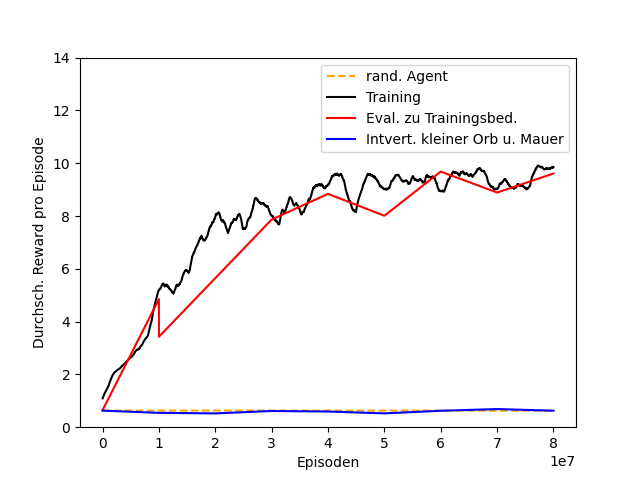
\includegraphics[scale=0.5]{abb/_graphen/semChange_mauerklOrb_80Mio_15act_training_}
        \caption{Evaluation zu Trainingsbed. und mit Invertierung der Mauer und kl. Orbs}
        \label{fig:semChange_mauerklOrb_80Mio_15act_training_}
    \end{minipage}
\end{figure}
\begin{center}
 \begin{table}[htp!]
 \begin{center}
  \begin{tabular}{ l c c c }
    \hline
		               			& Zeitschritte & Anzahl Level & 	 Invertierung\\ \hline
     Training              			& 80 Mio       & unbeschr.	    & 	 keine \\ \hline
     Eval. zu Trainingsbed.		& -	        	     & 50		    &	 keine \\ \hline
     Eval. Invertierung		 	& -	        	     & 50		    &	 Maucher u. kl. Orbs \\ \hline
    \hline
  \end{tabular}
  \caption{Übersicht über geltende Rahmenbedingungen in Training und Evaluation - 13.}
  \label{tab:tab_durch_EXP_trainSetting13}
  \end{center}
 \end{table}
\end{center} 

\textbf{Diskussion:} Die Evaluation zu Trainingsbedingungen (Abbildung \ref{fig:semChange_mauerklOrb_80Mio_15act_training_}) unterstützt die bisher gezeigten Ergebnisse. Ein Agent schafft es innerhalb von 80 Mio. Zeitschritten und einer unbeschränkten Level-Anzahl im Training die Generalisierungslücke zu schließen. Diese Evaluation bestätigt die Ergebnisse des Experiments in \ref{subsec:absch_EXP_durch_reproduktion_generalisierung}. Dagegen schafft der Graph der Evaluation mit semantischer Invertierung schafft es zu keinem Zeitpunkt über den des Random-Agenten hinaus. Eine mögliche Erklärung hierfür wäre, dass diese Änderung der Pixel-Verteilung zu stark ist. Im Verhältnis gibt es am Anfang eines Levels mehr kleine Orbs als Mauern. Vertauscht man nun diese beiden Sprites ist das Verhältnis umgedreht, wodurch sich die Pixel-Verteilung eines Frames stark verschiebt. Aufgrund dieser drastischen Änderung kann die Feature Extraction Pipeline die korrekten Features nicht mehr bereitstellen, um ein unbekanntes Level erfolgreich abzuschließen. Der folgende Paragraph beschreibt ein Experiment welches darauf aus ist, trotz semantischer Invertierung die Verschiebung der Pixel-Verteilung möglichst klein zu belassen.

\paragraph{Antwort: Set 3, Punkt 1}
Die Antwort auf diese Frage ist klar. Der Agent ist zu keinem Zeitpunkt besser als der Random-Agent. Somit ist die visuelle semantische Invertierung der Sprites des kleinen Orbs und der Mauern eine unüberwindbare Hürde für den Agenten. Der Agent ist mit seinem Grad an Generalisierung nicht in der Lage, in der Evaluation zu assimilieren. 

\paragraph{Invertierung - Geist und gr. Orbs}
Dieser Paragraph beschreibt Experimente mit der visuellen semantischen Invertierung der großen Orbs und der Geister. Hier wird derselbe Agent wie im Paragraphen zuvor verwendet. Dieses Experiment ist darauf aus die Veränderung der Pixel-Verteilung möglichst klein zu belassen. Da es sowohl drei Geister als auch drei große Orbs gibt, bieten sich diese beiden Spielelemente an, um auf diese Weise vertauscht zu werden. Wie in \ref{absch_RL_chaser} definiert haben die Geister in Chaser vier verschiedene States. Zwei dieser States (killing- und tödlich-State) haben Animation aus drei Sprites. Um die Pixel-Verteilung dieser Invertierung möglichst gering zu halten, sind die Geister auf ein einziges Sprite, während dieser beiden States, restriktiert. Die Sprites der anderen beiden States (idle-, verletzlich-State) bleiben unverändert. Somit stellt diese Invertierung keine Veränderung der Pixel-Verteilung des Agenten-Inputs dar. Wie zuvor stellt der schwarze Graph das Training dar und der rote die Evaluation zu Trainings-Bedingungen. Training und Evaluation zu Trainings-Bedingungen sind dieselben Graphen wie in Abbildung \ref{fig:semChange_mauerklOrb_80Mio_15act_training_}. 

Ein Bild des Agenten-Inputs kann dem Anhang entnommen werden (\ref{anh_env_bilder_chaser}, Titel \emph{Sprite-Tausch: großer Orb u.
Geist}). 

\begin{figure}[htp!]
   \centering
   \captionsetup{width=0.60\linewidth} 
    \begin{minipage}{0.48\linewidth}
        \centering\
        \textbf{Invertierung Mauer u. kleine Orbs}\par\medskip
        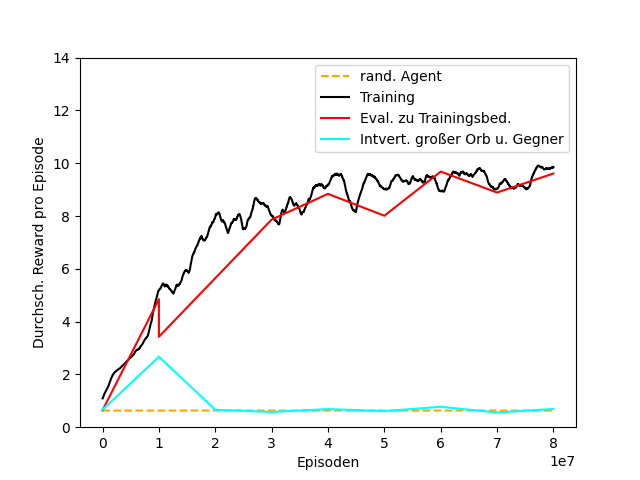
\includegraphics[scale=0.5]{abb/_graphen/semChange_geistGrOrb_80Mio_15act_training_}
        \caption{Evaluation zu Trainingsbed. und mit Invertierung der Geister und gr. Orbs}
        \label{fig:semChange_geistGrOrb_80Mio_15act_training_}
    \end{minipage}
\end{figure}
\begin{center}
 \begin{table}[htp!]
 \begin{center}
  \begin{tabular}{ l c c c }
    \hline
		               			& Zeitschritte & Anzahl Level & 	 Invertierung\\ \hline
     Training              			& 80 Mio       & unbeschr.	    & 	 keine \\ \hline
     Eval. zu Trainingsbed.		& -	        	     & 50		    &	 keine \\ \hline
     Eval. Invertierung		 	& -	        	     & 50		    &	 Geister u. gr. Orbs \\ \hline
    \hline
  \end{tabular}
  \caption{Übersicht über geltende Rahmenbedingungen in Training und Evaluation - 14.}
  \label{tab:tab_durch_EXP_trainSetting13}
  \end{center}
 \end{table}
\end{center} 

\textbf{Diskussion:} Die Evaluation mit der semantischen Invertierung der Geister und den großen Orbs (hier in cyan) entspricht der Intuition, die das vorangegangene Experiment suggeriert. Wie zuvor oszilliert die Performance des Agenten der Checkpoints 20 bis 80 Mio. eng um den Random-Agenten. Lediglich der Checkpoint bei 10 Mio. Zeitschritten weist einen Reward, höher als der des Random-Agenten, in Höhe von $2,67$ auf. Dieser Checkpoint schafft 10\% der Evaluations-Level. Diese semantische Invertierung ist in diesem Environment die mit den geringsten Veränderungen der Pixel-Verteilung und dennoch erreicht der Agent keinen durchschnittlichen Reward $\geq 10$.

\paragraph{Antwort: Set 3, Punkt 2}
Die Antwort dieses Experiments ist ebenso klar zu beantworten, wie die des vergangenen Experiments. Auch wenn der Reward des Agent beim Checkpoint bei 10 Mio. Zeitschritten überhalb dem des Random-Agenten ist, so liegen alle anderen Checkpoints nahe um den Reward des Random-Agenten. Der Agent scheitert somit eindeutig in der Evaluation. Eine mögliche Erklärung für den Ausreißer bei 10 Mio. ist, dass der Object Recognition Layer zu diesem Zeitpunkt im Training noch nicht so stark overfitted, wie bei den folgenden Checkpoints. Aufgrund dessen ist der Agent in der Lage in dieser veränderten Umgebung zu assimilieren und zielführende Entscheidungen zu treffen. 
















\newpage












